%-------------------------------------------------------------------------
%-------------------------------------------------------------------------
%-------------------------------------------------------------------------

\chapter[Interview Study\texorpdfstring{:\\ Visualizing Dimensionally Reduced Data: Interviews with Analysts and a Classification of Task Sequences}{}]{Interview Study\texorpdfstring{:\\ \large{Visualizing Dimensionally Reduced Data: Interviews with Analysts and a Classification of Task Sequences}}{}}
\label{ch:drvistasks}

%-------------------------------------------------------------------------
%-------------------------------------------------------------------------
%-------------------------------------------------------------------------

% \begin{epigraph}
%     \item (quote needed)
% \end{epigraph}

\footnote{This chapter is a slightly modified version of our paper {\it Visualizing Dimensionally Reduced Data: Interviews with Analysts and a Characterization of Task Sequences} by Matthew Brehmer, Michael Sedlmair, Stephen Ingram, and Tamara Munzner; in Proceedings of the ACM Workshop on Beyond Time and Errors: Novel Evaluation Methods For Information Visualization (BELIV 2014), p.1-8~\cite{Brehmer2014b}. \url{http://dx.doi.org/10.1145/2669557.2669559}.}We characterize five task sequences\index{task!task sequence} related to visualizing dimensionally reduced\index{dimensionality reduction (DR)} data, drawing from data collected from interviews with ten data analysts from different application domains, and from our understanding of the technique literature.
Our classification of visualization task sequences\index{task!task sequence} for dimensionally reduced\index{dimensionality reduction (DR)} data fills a gap created by the abundance of proposed techniques and tools that combine high-dimensional data\index{high-dimensional data} analysis, dimensionality reduction (DR), and visualization, and is intended to be used in the design and evaluation\index{evaluation} of future techniques and tools.
We discuss implications for the evaluation\index{evaluation} of existing work practices\index{work domain analysis}, for the design of controlled experiments, and for the analysis of post-deployment field observations.

%-------------------------------------------------------------------------
%-------------------------------------------------------------------------

\section{Motivation}
\label{drvistasks:intro}

%-------------------------------------------------------------------------
%-------------------------------------------------------------------------

\ac{DR}\index{dimensionality reduction (DR)} is the process of reducing a dataset with many dimensions to a lower-dimensional representation that retains most of its important structure. 
It has been an active research area throughout several decades and across many domains, from its origins in psychology~\cite{Torgerson1952,Young1938} through statistics~\cite{Buja2002} to machine learning\index{machine learning}
~\cite{Jain2000,Tenenbaum2000,VanderMaaten2008} and visualization~\cite{Ingram2010,Ingram2009,Johansson2009,Yang2003}.

While many techniques and tools combining \ac{DR}\index{dimensionality reduction (DR)} with visualization have been proposed, there is still no perfect automated solution that will generate the most effective visual encoding\index{visual encoding} for every situation. 
Analysts are faced with complex choices between alternative \ac{DR}\index{dimensionality reduction (DR)} techniques and between different visualization techniques for analyzing the resulting data.
These choices are strongly dictated by the analysts' data and tasks~\cite{Tatu2010a}\index{task}. 
The statistics and machine learning\index{machine learning} communities have provided extensive classifications of \ac{DR}\index{dimensionality reduction (DR)} techniques based on data and technique characteristics~\cite{Cunningham2008,France2011,Guyon2003,Jain2000,VanderMaaten2009,Witten2011}.
In contrast, there is very little that is explicitly stated about the characteristics of tasks\index{task} that analysts engage in when visually analyzing dimensionally reduced\index{dimensionality reduction (DR)} data. 
To guide designers, analysts, and those who conduct evaluations\index{evaluation} of techniques and tools, a better understanding of these tasks\index{task} is essential.

%-|-|-|-|-|-|-|-|-|-|-|-|-|-|-|-|-|-|-|-|-|-|-|-|-|-|-|-|-|-|-|-|-|-|-|-|-

\begin{figure}
	\centering
	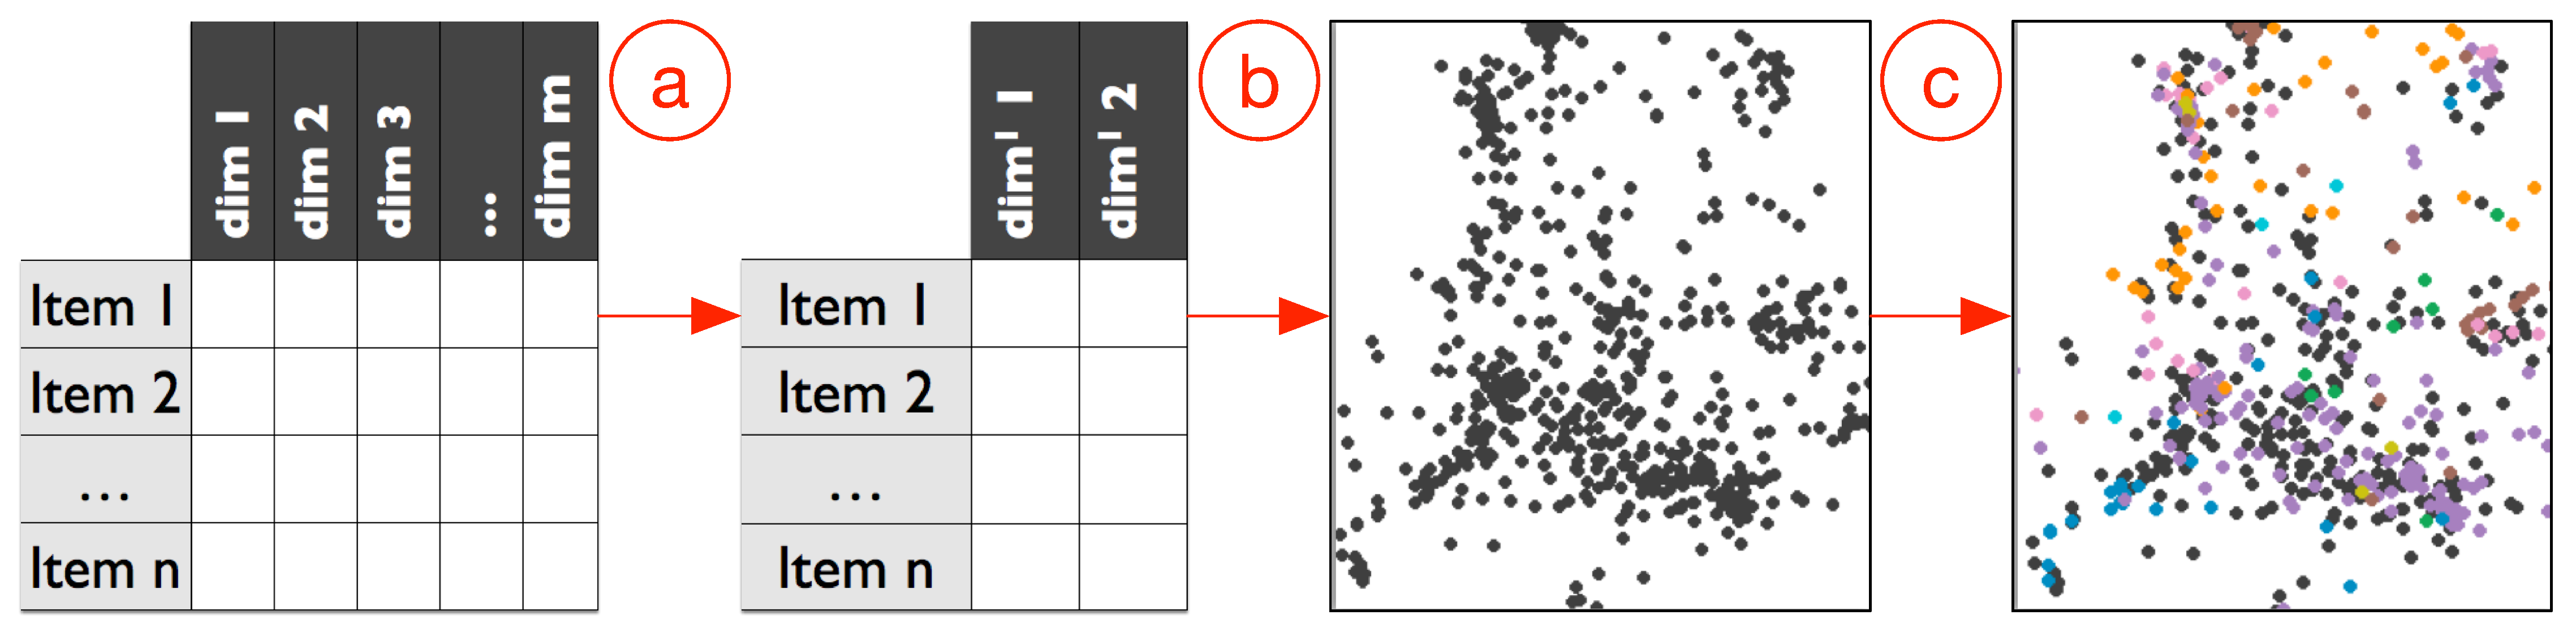
\includegraphics[width=\textwidth]{figures/drvizsequence.eps}
	\caption
	[
	    A task sequence involving dimensionally reduced data.
	]
	{
    	A task sequence involving dimensionally reduced data. (a) Data is reduced to two dimensions; (b) {\tt encoded} in a scatterplot to {\tt verify} visible clusters; and (c) colour-coded according to preexisting class labels to \textsl{match} clusters and classes.
	}
	\centering
	\label{drvistasks:fig:drvizsequence}
\end{figure} 

%-|-|-|-|-|-|-|-|-|-|-|-|-|-|-|-|-|-|-|-|-|-|-|-|-|-|-|-|-|-|-|-|-|-|-|-|-

The contribution of this chapter is a classification of five task sequences\index{task!task sequence} related to the visualization of dimensionally reduced\index{dimensionality reduction (DR)} data: {\it naming synthesized dimensions}, {\it mapping a synthesized dimension to original dimensions}, {\it verifying clusters}, {\it naming clusters}, and  {\it matching clusters and classes}. 
In the last of these sequences\index{task!task sequence}, illustrated in \autoref{drvistasks:fig:drvizsequence}, an analyst uses \ac{DR}\index{dimensionality reduction (DR)} and scatterplots\index{visual encoding!scatterplot} to verify\index{{\tt discover}} clusters, and then match them with existing classes.
Our classification is based on an in-depth analysis of ten interviews with analysts who use \ac{DR}\index{dimensionality reduction (DR)} for visualizing their data, as well as on a literature review of papers that apply \ac{DR}\index{dimensionality reduction (DR)} for the purpose of data visualization.
Our analysis\index{task!task analysis} framework is our typology\index{task!task typology} of abstract tasks\index{task!task abstraction} proposed in \autoref{ch:typology}.
Our typology\index{task!task typology} allows practitioners to characterize task sequences\index{task!task sequence} based on observed work practices\index{work domain analysis}, occurring in requirements gathering activities and in field evaluations\index{evaluation} of deployed tools.

%-------------------------------------------------------------------------
%-------------------------------------------------------------------------

\section{Related Work}
\label{drvistasks:rw}

%-------------------------------------------------------------------------
%-------------------------------------------------------------------------

\bstart{Classifying tasks}
The systematic analysis\index{task!task analysis} of worker activities\index{work domain analysis} and tasks\index{task} is a critical process in the design and evaluation\index{evaluation} of technology, and task analysis\index{task!task analysis} frameworks appear in many different fields, including human factors and ergonomics~\cite{Vicente1999}, \ac{HCI}\index{human-computer interaction (HCI)}~\cite{Mullins1993}, and visualization, including the typology\index{task!task typology} of tasks proposed in \autoref{ch:typology}.

While many classifications of visualization tasks\index{task} are agnostic to datatype, some address specific types of data~\cite{Shneiderman1996}, such as network data~\cite{Lee2006}, time-oriented data~\cite{Lammarsch2012}\index{time-oriented data}, and tabular data~\cite{Henry2006}.
As we discussed in \autoref{typology:rw:taxonomies} and in \citet{Meyer2015}, datatype-specific task\index{task} classifications consider a specific set of {\it data abstractions}\index{data abstraction}, facilitating a mapping to appropriate visual encoding\index{visual encoding} and interaction\index{interaction} design choices.
A datatype-specific task\index{task} classification of tasks\index{task} is also critical for evaluation\index{evaluation}, such as when specifying tasks\index{task} to be performed by participants in controlled experiments.
In this chapter, we propose a datatype-specific classification of task sequences\index{task!task sequence} for {\it dimensionally reduced}\index{dimensionality reduction (DR)} data. 

Classifications of tasks\index{task} are often based on their authors' own experience in conjunction with a thorough consideration of the literature~\cite{Amar2004,Shneiderman1996}, while others are based on observations of human behaviour in controlled laboratory settings~\cite{Amar2005}. 
In contrast, our classification of task sequences\index{task!task sequence} is primarily based on an interview study with analysts working with their own data~\cite{McGrath1995}, allowing us to ground our findings in real data analysis practices.

\begin{sloppypar}
\bstart{Mapping tasks to design choices for high-dimensional data analysis}
There are many approaches that combine analysis of high-dimensional data\index{high-dimensional data}, \ac{DR}\index{dimensionality reduction (DR)}, and visualization, including some developed by our research group~\cite{Ingram2010,Ingram2009,Williams2004}.
While there are existing classifications of high-dimensional data\index{high-dimensional data} analysis techniques~\cite{Bertini2011} and of dimensionally reduced\index{dimensionality reduction (DR)} data~\cite{Sedlmair2012a}, the mapping between data, tasks\index{task}, and appropriate design choices remains unclear~\cite{Tatu2010a}. 
This problem is particularly apparent when designing to accommodate {\it workflows}\index{workflows}, or instantiations of task sequences\index{task!task sequence} within software tools for high-dimensional data\index{high-dimensional data} analysis~\cite{Ingram2010,Johansson2009}.
\end{sloppypar}

One task\index{task} for dimensionally reduced\index{dimensionality reduction (DR)} data is that of matching clusters and categorical classes given with the data, discussed below in \autoref{drvistasks:tasks:clusters}. 
Based on findings from an empirical data study, we previously identified effective visual encoding design choices that support this task~\cite{Sedlmair2013}, and we called for similar work to be done for other tasks\index{task} relating to dimensionally reduced\index{dimensionality reduction (DR)} data.
Our classification of task sequences\index{task!task sequence} moves us closer to this goal.

\bstart{Expert judgments and dimensionally reduced\index{dimensionality reduction (DR)} data}
We are aware of one other study involving expert analysts' interpretations of visualized dimensionally reduced\index{dimensionality reduction (DR)} data, though they do not share our explicit examination of analysts' domain problems and tasks\index{task}: \citet{Lewis2012} asked expert and novice analysts in a controlled lab setting to subjectively rate the value of two-dimensional scatterplots\index{visual encoding!scatterplot} of seven dimensionally reduced\index{dimensionality reduction (DR)} datasets, generated using nine different \ac{DR}\index{dimensionality reduction (DR)} techniques. 
Their findings showed that experts were more consistent than novices in their positive and negative ratings.
Judging the value or quality of a visual encoding\index{visual encoding} of dimensionally reduced\index{dimensionality reduction (DR)} data should occur regardless of task\index{task}, and analysts can additionally leverage automated quality metrics based on human perception~\cite{Albuquerque2010a,Bertini2011}. 
In our study, the domain experts we interviewed varied in terms of their perceived understanding of \ac{DR}\index{dimensionality reduction (DR)}; furthermore, we sought to characterize experts' tasks\index{task} and activities in naturalistic settings, rather than in a controlled lab study.

%-------------------------------------------------------------------------
%-------------------------------------------------------------------------

\section{Research Process}
\label{drvistasks:methods}

%-------------------------------------------------------------------------
%-------------------------------------------------------------------------

Our methodological choice was motivated by a vibrant thread of work in the visualization community using qualitative methods in general~\cite{Carpendale2008,Isenberg2008,Tory2008}, and interview studies in particular~\cite{Kandel2012,Kang2011}\footnote{We elaborate on the evolution of our methodology and the foci of our analysis in \autoref{app:drvistasks:methodology}.}.

\bstart{Data collection}
Between 2010 and 2012, we interviewed nineteen data analysts working in academic and industry settings, representing over a dozen domains, spanning the natural sciences, computer science, policy analysis\index{policy analysis}, and investigative journalism\index{journalism}. 
These analysts were recruited from our extended personal and professional networks via snowball sampling, and they were known to work with high-dimensional data\index{high-dimensional data}.
These interviews were semi-structured, lasting in duration from one to four hours\footnote{In \autoref{app:drvistasks:interview-list}, we indicate that we conducted twenty-four interviews in total, as five analysts were interviewed twice; see \autoref{tab:interviews}.}; some of these interviews were more akin to contextual inquiries~\cite{Holtzblatt1993}\index{evaluation!contextual inquiry}, occurring at the analyst's workplace, while others were performed in our department or via teleconference.

We discussed the analysts' domain context, their data analysis goals, and their data; we also asked more specific questions about how they transformed their data and their use of \ac{DR}\index{dimensionality reduction (DR)} and visualization techniques\footnote{The interview foci and questions can be found in \autoref{app:drvistasks:interview-foci}}.
We also collected artifacts from these analysts, including their published papers and theses, their unpublished manuscripts, screenshots of their visualized data, and in some cases, even their data.

\bstart{Data analysis}
We alternated between data collection and analysis, progressing from {\it initial} to {\it focused} coding\index{coding (qualitative data analysis)} of the data~\cite{Charmaz2006}\footnote{Example artefacts from this data analysis process can be found in \autoref{app:drvistasks:analysis-examples}.}\index{grounded theory}.

In this chapter we concentrate our attention on the ten analysts who (a) specifically used dimensional synthesis \ac{DR}\index{dimensionality reduction (DR)!dimensional synthesis} algorithms\index{algorithms} in analyzing their high-dimensional data\index{high-dimensional data}, and who (b) also visualized their dimensionally reduced\index{dimensionality reduction (DR)} data.

To analyze the data that we collected from these ten interviews, we used our typology\index{task!task typology} of abstract visualization tasks\index{task!task abstraction}, proposed in \autoref{ch:typology}.
Our typology\index{task!task typology} distinguishes {\it why}\index{{\tt why}} data is being visualized at multiple levels of abstraction\index{task!task abstraction}, {\it what}\index{{\tt what}} {\tt inputs}\index{{\tt input}} and {\tt outputs}\index{{\tt output}} a task\index{task} may have, as well as {\it how}\index{{\tt how}} a task\index{task} is supported by visual encoding\index{visual encoding} and interaction\index{interaction} design choices. 
This lens allowed us to focus on a subset of our findings from the standpoint of visualization design and evaluation\footnote{The previous interpretations of our findings are documented in \autoref{app:drvistasks:previous-interpretations}. We initially focused on characterizing \ac{DR}\index{dimensionality reduction (DR)} techniques, people who use them, their tasks\index{task}, and their challenges~\cite{Sedlmair2012b}. 
Later, we narrowed our focus to that of \ac{DR}\index{dimensionality reduction (DR)} techniques and related tasks\index{task} (see \autoref{app:drvistasks:dritw}). 
In this chapter, our focus is even narrower, on tasks\index{task} relating to the visualization of dimensionally reduced data following the use of dimensional synthesis \ac{DR} techniques.}\index{evaluation}, culminating in the task sequences\index{task!task sequence} presented in \autoref{drvistasks:tasks}.
In Section \ref{drvistasks:typology}, we revisit the typology\index{task!task typology} and illustrate how it can describe our five task sequences\index{task!task sequence}. 
%RR: p. 51, bottom. Using the typology to "better interpret" the data. Although any reference frame causes some things to be emphasized (and thus, better interpreted), it also causes others to be de-emphasized, or even lost. What's lost here? More generally, what are the weakest aspects of this approach? Could they be fixed, given enough time?

Finally, we enriched our analysis with further examples from the literature.
We specifically sought papers that report on applications where \ac{DR}\index{dimensionality reduction (DR)} and visualization were performed in conjunction for analysis, and we consider these applications with respect to the task sequences\index{task!task sequence} we characterized. 

%-------------------------------------------------------------------------
%-------------------------------------------------------------------------

\section{Task Sequences}
\label{drvistasks:tasks}

%-------------------------------------------------------------------------
%-------------------------------------------------------------------------

%-|-|-|-|-|-|-|-|-|-|-|-|-|-|-|-|-|-|-|-|-|-|-|-|-|-|-|-|-|-|-|-|-|-|-|-|-

\begin{figure}
	\centering
	\begin{subfigure}[t]{\textwidth}
	    \centering
        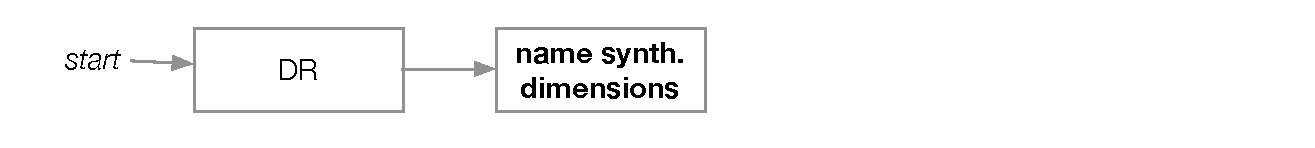
\includegraphics[height=1cm]{figures/drviztasks-name-dims.eps}
    \end{subfigure}
    ~
    \begin{subfigure}[t]{\textwidth}
	    \centering
        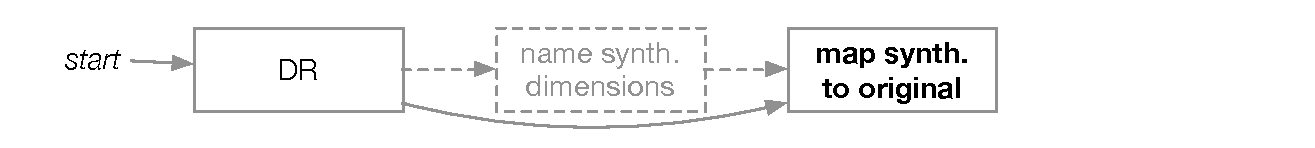
\includegraphics[height=1cm]{figures/drviztasks-map-dims.eps}
    \end{subfigure}
    ~
    \begin{subfigure}[t]{\textwidth}
	    \centering
        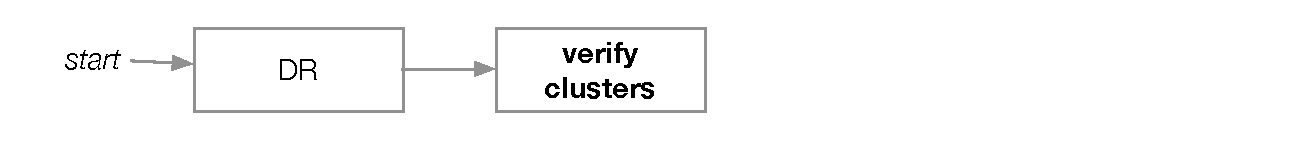
\includegraphics[height=1cm]{figures/drviztasks-identify-clusters.eps}
    \end{subfigure}
    ~
    \begin{subfigure}[t]{\textwidth}
	    \centering
        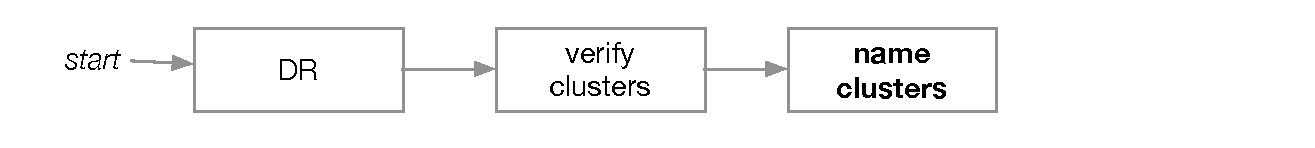
\includegraphics[height=1cm]{figures/drviztasks-name-clusters.eps}
    \end{subfigure}
    ~
    \begin{subfigure}[t]{\textwidth}
	    \centering
        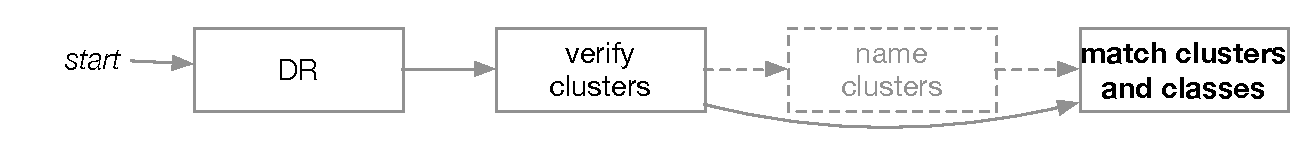
\includegraphics[height=1cm]{figures/drviztasks-match-clusters.eps}
    \end{subfigure}
	\caption
	[
	    Five task sequences that involve visualizing dimensionally reduced data.
	]
	{
    	
    	Five task sequences that involve visualizing dimensionally reduced data. Individual tasks are described using our typology in \autoref{drvistasks:fig:drviztasks}.
	}
	\centering
	\label{drvistasks:sequences}
\end{figure}

%-|-|-|-|-|-|-|-|-|-|-|-|-|-|-|-|-|-|-|-|-|-|-|-|-|-|-|-|-|-|-|-|-|-|-|-|-

We have identified five task sequences\index{task!task sequence} related to dimensionally reduced\index{dimensionality reduction (DR)} data.
In this section, we describe each task sequence\index{task!task sequence} and illustrate the sequence\index{task!task sequence} in \autoref{drvistasks:sequences}. 
Each is named after the terminal task\index{task} appearing in the sequence\index{task!task sequence}.
We also comment on how these task sequences\index{task!task sequence} arose in our interviews, and which visualization techniques were used to address these sequences\index{task!task sequence}. 
These task sequences\index{task!task sequence} are not exclusive: some analysts performed multiple task sequences\index{task!task sequence} in the course of their work.
This descriptive survey of analysts' data, task sequences\index{task!task sequence}, and visualization is summarized in \autoref{drvistasks:tab:summary}. 
The dataset sizes being investigated by these analysts ranged from dozens to over a million dimensions, and from hundreds to hundreds of thousands of items.  

%-|-|-|-|-|-|-|-|-|-|-|-|-|-|-|-|-|-|-|-|-|-|-|-|-|-|-|-|-|-|-|-|-|-|-|-|-

\begin{table}\renewcommand{\arraystretch}{1.2}\addtolength{\tabcolsep}{-1pt}
	\begin{center}
	\tiny
	\begin{tabular}{@{}|l|>{\RaggedRight}p{0.125\textwidth}l|*{2}c|*{5}c|*{7}c|@{}}

		\hline

		\cellcolor{blue!15} {\bf Case}
		& \multicolumn{2}{c|}{\cellcolor{blue!15} {\bf Data}} 
		& \multicolumn{2}{c|}{\cellcolor{blue!15} {\bf DR}} 
		& \multicolumn{5}{c|}{\cellcolor{blue!15} {\bf Task Sequence}} 
		& \multicolumn{7}{c|}{\cellcolor{blue!15} {\bf Visualization Techniques}}

		\\

		\hline

		\rowcolor{blue!15}

		{\rot{\bf ID}}

		& {\rot{\bf Description}} & {\rot{\bf \# Dims x Items}}

		& {\rot{\bf Linear}} & {\rot{\bf Non-Linear}}

		& {\rot{\it Name Dimensions}} & {\rot{\it Map Dimensions}} & {\rot{\it Verify Clusters}} & {\rot{\it Name Clusters}} & {\rot{\it Match Clusters}}

		& {\rot{\bf 2D Scatterplots}\index{visual encoding!scatterplot}} & {\rot{\bf 3D Scatterplots}\index{visual encoding!scatterplot!3D scatterplot}} & {\rot{\bf SPLOMs}}\index{visual encoding!scatterplot!scatterplot matrix (SPLOM)} & {\rot{\bf Scree plots}\index{visual encoding!scree plot}} & {\rot{\bf Graph / Tree}}\index{visual encoding!tree}\index{visual encoding!node-link graph} & {\rot{\bf Correl. matrix}}\index{visual encoding!matrix!correlation matrix} & {\rot{\bf Heat maps}\index{visual encoding!heat map}}

		\\

		\hline

		\refstepcounter{rownumber} 
		\therownumber\label{drvistasks:analyst:JB} %Music / Jennifer Büttgen

% 		& HCI

		& usage logs from online music service & 48 x 310 %10\textsuperscript{1} &  10\textsuperscript{2} %48, 310

		& \OK & 

		& \OK & \OK & \OK & \OK & \OK 
		%[i] \ac{DR}\textsuperscript{1} $\rightarrow$ {\it name synth. dims} $\rightarrow$ {\it map synth. to original }; [ii] \ac{DR}\textsuperscript{1} $\rightarrow$ {\it verify clusters} $\rightarrow$ {\it name clusters} $\rightarrow$ {\it match clusters and classes}

		& \OK & & \OK & & & & 
		%2D scatterplots, \ac{SPLOM}s

		\\

		\rowcolor{gray!15}

		\refstepcounter{rownumber} 
		\therownumber\label{drvistasks:analyst:HL} %Search / Heidi Lam

% 		& HCI

		& aggregated search engine metrics  & 12--31 x 1,463%10\textsuperscript{1} & 10\textsuperscript{3} % 12-31,1463

		& \OK & \OK 

		& \OK & \OK & \OK & \OK & \OK 
		%[i] \ac{DR}\textsuperscript{1,2} $\rightarrow$ {\it name synth. dims} $\rightarrow$ {\it map synth. to original }; [ii] \ac{DR}\textsuperscript{1,2} $\rightarrow$ {\it verify clusters} $\rightarrow$ {\it name clusters} $\rightarrow$ {\it match clusters and classes}

		& \OK & & & & & & 
		%2D scatterplots

		\\

		\refstepcounter{rownumber} 
		\therownumber\label{drvistasks:analyst:CM} %BoatAct / Cindy Marven

% 		& PA

		& recreational boating survey data & 39 x 543 %10\textsuperscript{1} & 10\textsuperscript{2} %39, 543

		& \OK & \OK

		& & \OK & \OK & \OK &
		%[i] \ac{DR}\textsuperscript{1,2} $\rightarrow$ {\it map synth. to original }; [ii] \ac{DR}\textsuperscript{1,2} $\rightarrow$ {\it verify clusters} $\rightarrow$ {\it name clusters}

		& \OK & \OK & \OK & & \OK & & 
		% 2D scatterplots, 3D scatterplots, \ac{SPLOM}s, dendrograms

		\\ 

		\rowcolor{gray!15}

		\refstepcounter{rownumber} 
		\therownumber\label{drvistasks:analyst:CN} %EpiGen / Cydney Nielsen

% 		& BI

		& protein region data & 160 x 10--100K%10\textsuperscript{2} & 10\textsuperscript{5} % 160, 10-100k

		& \OK & \OK

		& & \OK & \OK & \OK &  
		%[i] \ac{DR}\textsuperscript{1,2} $\rightarrow$ {\it map synth. to original }; [ii] \ac{DR}\textsuperscript{1,2} $\rightarrow$ {\it verify clusters} $\rightarrow$ {\it name clusters}

		& & & \OK & & & & \OK %, {\it Spark}~\cite{Nielsen2012}
		% \ac{SPLOM}s, density plots, heatmaps %, {\it Spark}~\cite{Nielsen2012}

		\\

		\refstepcounter{rownumber} 
		\therownumber\label{drvistasks:analyst:ST} %Polymers / Sid Thakur

% 		& CH

		& polymer molecule feature vectors & 1K x 10K %10\textsuperscript{3} & 10\textsuperscript{4} % 1k,10k

		& \OK & \OK

		& & & \OK & \OK & 
		
		% \ac{DR}\textsuperscript{1,2} $\rightarrow$ {\it verify clusters} $\rightarrow$ {\it name clusters}

		& \OK & & & & & \OK & \OK
		% 2D scatterplots, heatmaps, correlation matrices

		\\

		\rowcolor{gray!15}

		\refstepcounter{rownumber} 
		\therownumber\label{drvistasks:analyst:HY} %Concept / Hong Yi

% 		& SN

		& bibliometric co-occurrence matrix & 20K x 20K %10\textsuperscript{4} & 10\textsuperscript{4} % 20k

		& \OK & \OK

		& & & \OK & \OK &
		%1. \ac{DR}\textsuperscript{1,2} $\rightarrow$ {\it name synth. dims}; 2. 
		%\ac{DR}\textsuperscript{1,2} $\rightarrow$ {\it verify clusters} $\rightarrow$ {\it name clusters}

		& \OK & & \OK & \OK & & \OK &
		% 2D scatterplots, {\it DimStiller}~\cite{Ingram2010} (\ac{SPLOM}s, correlation matrices)

		\\

		\refstepcounter{rownumber} 
		\therownumber\label{drvistasks:analyst:KA} %MoCap / Kerem Altun

% 		& HCI 

		& human motions from multiple sensors & 1,170 x 9,120 %10\textsuperscript{3} & 10\textsuperscript{3} %1170, 9120

		& \OK & 

		& & & \OK & & \OK  
		%\ac{DR}\textsuperscript{1} $\rightarrow$ {\it verify clusters} $\rightarrow$ {\it match clusters and classes}

		& \OK & \OK & & & & &
		% 2D scatterplots, interactive 3D scatterplots

		\\

		\rowcolor{gray!15}

		% H %ChemRel / Klaus Dress

		% & Computational chemistry

		% & \ac{DR}\textsuperscript{2} $\rightarrow$ {\it verify clusters} $\rightarrow$ {\it match clusters and classes}

		% % & non-linear

		% & correlation matrices, {\it Spotfire}~\cite{Spotfire}, {\it Tableau}~\cite{Tableau}

		% \\

		\refstepcounter{rownumber} 
		\therownumber\label{drvistasks:analyst:AC} %ProstCan / Anamaria Crisan

% 		& BI

		& genomic, clinical data from patients & 1.4M x 600 %10\textsuperscript{6} & 10\textsuperscript{2} %1.4M, 600

		& \OK & \OK

		& & & \OK & & \OK
		%\ac{DR}\textsuperscript{1,2} $\rightarrow$ {\it verify clusters} $\rightarrow$ {\it match clusters and classes}

		& \OK & \OK & & & & &
		% 2D scatterplots, 3D scatterplots

		\\

		\refstepcounter{rownumber} 
		\therownumber\label{drvistasks:analyst:DH} %SeqAln / Des Higgins

% 		& BI

		& distance matrix of genome sequences & 100K x 100K %10\textsuperscript{5} & 10\textsuperscript{5} %100k

		& \OK & \OK

		& & & \OK & \OK & \OK
		%\ac{DR}\textsuperscript{1,2} $\rightarrow$ {\it verify clusters} $\rightarrow$ {\it name clusters} $\rightarrow$ {\it match clusters and classes}

		& \OK & \OK & \OK & & \OK & &
		% 2D scatterplots, 3D scatterplots, \ac{SPLOM}s, node-link graphs

		\\

		\rowcolor{gray!15}

		\refstepcounter{rownumber} 
		\therownumber\label{drvistasks:analyst:JS} %TxtDocs / Jonathan Stray

% 		& IJ

		& distance matrix of text documents & 10K x 10K %10\textsuperscript{4} & 10\textsuperscript{4} %10k

		&  & \OK

		& & & \OK & \OK & \OK
		%\ac{DR}\textsuperscript{2} $\rightarrow$ {\it verify clusters} $\rightarrow$ {\it name clusters} $\rightarrow$ {\it match clusters and classes}

		& \OK & & & & \OK & &
		% 2D scatterplots, node-link graphs

		\\

		\hline

		\rowcolor{blue!15}

		{\bf Ref.}

% 		& 

		& 

		& %dims	
% 		& %items

		& %linear 
		& %non-linear

		& %name dims
		& %map dims
		& %verify clusters
		& %name clusters
		& %match clusters

		& %2D SPs
		& %3D SPs
		& %\ac{SPLOM}s
		& %scree plots
		& %node-link
		& %correl matrix
		& %heatmaps

		\\

		\hline

		\cite{Buja2002} %MorseCd
% 		\cite{Tenenbaum2000} %Faces
% 		\cite{Matusik2003} %BRDF
% 		\cite{Reveret2005} %Quadrup

% 		& 

		& distance matrix of Morse codes & 36 x 36 %10\textsuperscript{1} & 10\textsuperscript{1} %26

		& & \OK

		% & linear; non-linear

		&  \OK &  & \OK  & \OK  & 

		% \ac{DR}\textsuperscript{1,2} $\rightarrow$ {\it name synth. dims}

		&  \OK &  &  & & & &

		% 2D scatterplots with text labels and inter-class connections 

		\\

		\rowcolor{gray!15}

		\cite{Matusik2003} %BRDF

% 		& 

		& BRDF reflectance model & 4.36M x 104 %10\textsuperscript{6} & 10\textsuperscript{2} %4364000, 104

		& \OK & \OK 

		% & linear; non-linear

		&  \OK &  &  &  & 

		% \ac{DR}\textsuperscript{1,2} $\rightarrow$ {\it name synth. dims}

		& \OK &  &  & \OK & & &

		% 2D scatterplots with text labels 

		\\

		\cite{Reveret2005} %Quadrup

% 		& 

		& quadruped skeleton models & 348--406 x 9 %10\textsuperscript{2} & 10\textsuperscript{1} %348-406, 9

		& \OK &
		%linear

		& \OK & & & &
		% \ac{DR}\textsuperscript{1} $\rightarrow$ {\it name synth. dims}

		% & linear

		& & & & \OK & & &
		% Scree plot

		\\

		\rowcolor{gray!15}

		\cite{Tenenbaum2000} %Faces

% 		& 

		& 64 x 64 px images & 4,096 x 698--1K %10\textsuperscript{3} & 10\textsuperscript{2} %4096, 698-1000

		& & \OK
		% non-linear

		& \OK & & & &
		% \ac{DR}\textsuperscript{2} $\rightarrow$ {\it name synth. dims}

		& \OK & & & \OK & & &
		% 2D scatterplots with image glyphs adjacent to points

		\\

		% \cite{Bronstein2006a} %ArtShp

		% & Computer graphics

		% & \ac{DR}\textsuperscript{2} $\rightarrow$ {\it verify clusters} $\rightarrow$ {\it match clusters and classes}

		% % & non-linear

		% & similarity matrix

		% \\

		\hline

	\end{tabular}
	\caption
	[
	    A summary of task sequences performed by the ten analysts that we interviewed and found in papers discussing \ac{DR} and visualization.
	]
	{
	    {\it Top}: A summary of task sequences performed by the ten analysts that we interviewed, along with the visualization techniques(s) used to perform these tasks sequences. 
	   % *Domains: HCI = Human-Computer Interaction; PA = Policy Analysis; BI = Bioinformatics; CH = Chemistry; SN = Social Network Analysis; IJ = Investigative Journalism. 
	    {\it Bottom}: examples of task sequences in papers discussing \ac{DR} and visualization.
	} 
	\label{drvistasks:tab:summary}
	\end{center}
\end{table}

%-|-|-|-|-|-|-|-|-|-|-|-|-|-|-|-|-|-|-|-|-|-|-|-|-|-|-|-|-|-|-|-|-|-|-|-|-

\bstart{Dimensionality reduction}
All the task sequences\index{task!task sequence} we characterized begin with \ac{DR}\index{dimensionality reduction (DR)}.
In our context, we define \ac{DR}\index{dimensionality reduction (DR)} as a means\index{task!means} of dimensional synthesis\index{dimensionality reduction (DR)!dimensional synthesis}: a set of $m$ synthesized dimensions is {\tt derived}\index{{\tt derive}} from $n$ original dimensions, where $m$~\textless~$n$. 
Dimensional synthesis\index{dimensionality reduction (DR)!dimensional synthesis} techniques are commonly differentiated between {\it linear} and {\it non-linear}~\cite{Jain2000}. 
Linear techniques such as \ac{PCA}\index{dimensionality reduction (DR)!principal component analysis (PCA)}~\cite{Jolliffe2002} or classical \ac{MDS}\index{dimensionality reduction (DR)!multi-dimensional scaling (MDS)}~\cite{Torgerson1952,Young1938} produce\index{{\tt produce}} synthetic dimensions from linear projections of the original data. 
However, many datasets have an intrinsic structure that can only be revealed using non-linear techniques, such as Isomap~\cite{Tenenbaum2000}, \ac{t-SNE}\index{dimensionality reduction (DR)!t-distributed stochastic neighbor embedding (t-SNE)}~\cite{VanderMaaten2008}, or Glimmer \ac{MDS}\index{dimensionality reduction (DR)!multi-dimensional scaling (MDS)}~\cite{Ingram2009}.
Further distinction between linear and non-linear dimensional synthesis\index{dimensionality reduction (DR)!dimensional synthesis} is outside of the scope of this chapter, though we note that some techniques are more appropriate for verifying the existence of local cluster structure while others are more appropriate for identifying\index{{\tt identify}} global intrinsic dimensions (or {\it manifolds})~\cite{Lewis2012}.
In \autoref{drvistasks:tab:summary}, we note who used linear and non-linear \ac{DR}\index{dimensionality reduction (DR)}.

It is not our intent to catalog and differentiate the large body of \ac{DR}\index{dimensionality reduction (DR)} techniques; we will concentrate our analysis on their {\tt output}\index{{\tt output}}, asking {\it why}\index{{\tt why}} do analysts visualize these synthesized dimensions.

%-------------------------------------------------------------------------

\subsection{Dimension-Oriented Task Sequences}
\label{drvistasks:tasks:dims}

%-------------------------------------------------------------------------

We describe two task sequences\index{task!task sequence} that specifically relate to {\it synthesized} dimensions as generated by dimensional synthesis\index{dimensionality reduction (DR)!dimensional synthesis} \ac{DR}\index{dimensionality reduction (DR)} techniques: {\it naming synthesized dimensions} and {\it mapping synthesized to original dimensions}.
The verbs {\it name} and {\it map} were deliberately chosen and are defined using the vocabulary of our typology\index{task!task typology} in the following two subsections.

% %-------------------------------------------------------------------------

% \subsubsection{Name Synthesized Dimensions}
% \label{drvistasks:tasks:name-dims}

% %-------------------------------------------------------------------------

% \begin{figure}[!ht]
% 	\centering
% 	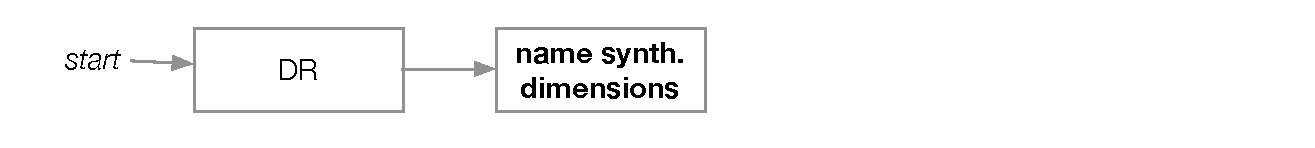
\includegraphics[width=\textwidth]{figures/drviztasks-name-dims.eps}
% 	\centering
% \end{figure} 

\bstart{Name synthesized dimensions}
Given a set of synthesized dimensions, an analyst may want to {\tt discover}\index{{\tt discover}} what these dimensions mean, to {\tt generate hypotheses}\index{{\tt discover}} about the semantics of these synthesized dimensions.
An analyst will {\tt browse}\index{{\tt browse}} the set of synthesized dimensions, and for each dimension of interest, she will {\tt browse}\index{{\tt browse}} items and their corresponding values; as a result, she may be able to {\tt identify}\index{{\tt identify}} the name of a synthesized dimension.

This task sequence\index{task!task sequence} was attempted by two of the analysts we interviewed (\ref{drvistasks:analyst:JB} and~\ref{drvistasks:analyst:HL} in \autoref{drvistasks:tab:summary}). 
Both worked in the field of \ac{HCI}\index{human-computer interaction (HCI)} and attempted to {\tt identify}\index{{\tt identify}} the intrinsic dimensions related to usage data collected about online search behaviour and music listening behaviour, respectively. 

A common approach, employed by both analysts, is to inspect data points plotted according to two synthesized dimensions in a two-dimensional scatterplot\index{visual encoding!scatterplot}, in which the analyst may be able to discern an interesting semantic relationship along the axes. 
In some cases, these scatterplots\index{visual encoding!scatterplot} are augmented with text labels containing categorical information, such as item name, annotated\index{{\tt annotate}} adjacent to a subset of the plotted points~\cite{Buja2002,Matusik2003,Tenenbaum2000} or available through interaction\index{interaction}. 
Tenenbaum~\etal's paper describing the Isomap algorithm~\cite{Tenenbaum2000} contains a particularly compelling example (reproduced in \autoref{drvistasks:fig:drviztasks-name-dims-tenenbaum}), in which each data point in a scatterplot\index{visual encoding!scatterplot} corresponds to an image of a face; a random sample of these images are displayed directly in the scatterplot\index{visual encoding!scatterplot} as thumbnails adjacent to their corresponding points.
Given this display, it is possible to discern names for the three synthesized dimensions resulting from dimensional synthesis\index{dimensionality reduction (DR)!dimensional synthesis}. 

\begin{figure}
	\centering
	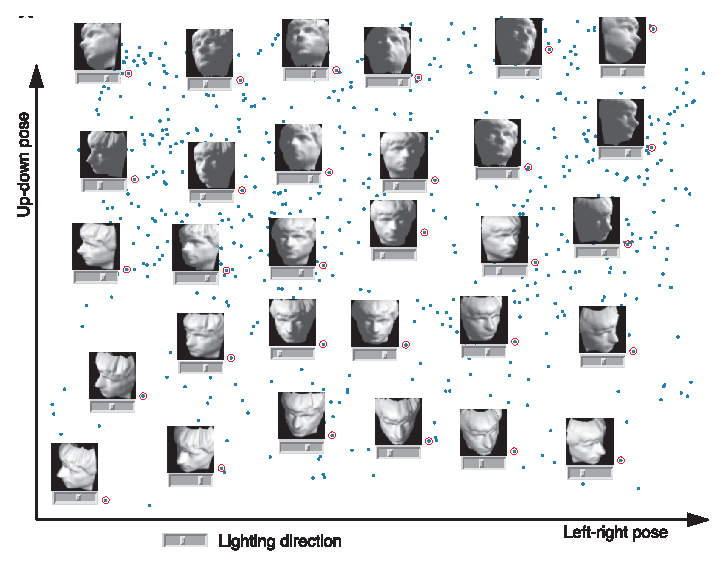
\includegraphics[width=\textwidth]{figures/drviztasks-name-dims-tenenbaum.eps}
	\caption
	[
	    A visual encoding of dimensionally reduced data, in which three synthesized dimensions have been identified.
	]
	{
    	 A visual encoding of dimensionally reduced data, in which three synthesized dimensions have been identified: \textsl{up-down pose} along the y-axis, \textsl{left-right pose} along the x-axis, and \textsl{lighting direction} indicated below each image.
    	 Figure from \citet{Tenenbaum2000} (\copyright~[2000] AAAS).
	}
	\centering
	\label{drvistasks:fig:drviztasks-name-dims-tenenbaum}
\end{figure} 

% %-------------------------------------------------------------------------

% \subsubsection{Map Synthesized to Original Dimensions}
% \label{drvistasks:tasks:map-dims}

% %-------------------------------------------------------------------------

% \begin{figure}[!ht]
% 	\centering
% 	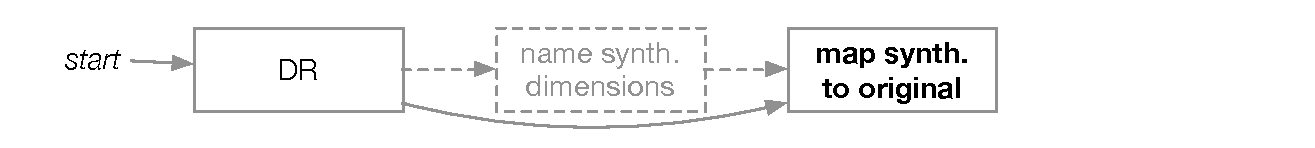
\includegraphics[width=\textwidth]{figures/drviztasks-map-dims.eps}
% 	\centering
% \end{figure} 

\bstart{Map synthesized to original dimensions}
Regardless of whether an analyst is interested in naming synthesized dimensions, another possible task sequence\index{task!task sequence} involves mapping synthesized dimensions back to original dimensions.
In the context of \ac{PCA}\index{dimensionality reduction (DR)!principal component analysis (PCA)}~\cite{Jolliffe2002}, this mapping is often referred to as the {\it loading} of the synthesized dimensions by the original dimensions.
Given a synthesized dimension, an analyst may want to {\tt discover}\index{{\tt discover}} this mapping. 
More specifically, the analyst may either {\tt verify}\index{{\tt discover}} a hypothesis that this mapping exists, or {\tt generate}\index{{\tt discover}} a new hypothesis about it. 
The analyst will {\tt browse}\index{{\tt browse}} items and their values along this synthesized dimension and {\tt compare}\index{{\tt compare}} these values to those along the set of original dimensions, looking for similarities and correlations.
This mapping could allow analysts to {\tt identify}\index{{\tt identify}} groups of correlated original dimensions.

Four of the analysts we interviewed attempted to perform this sequence\index{task!task sequence} of tasks; two of these analysts had previously attempted to name some of their synthesized dimensions.
\ref{drvistasks:analyst:JB} mapped her synthesized dimensions to a set of original dimensions in aggregated usage logs from an online music streaming service, while~\ref{drvistasks:analyst:HL} attempted the same task sequence\index{task!task sequence} with aggregate search engine metrics but was unable to confidently map any of her synthesized dimensions to her original dimensions. 
Both used two-dimensional scatterplots\index{visual encoding!scatterplot} to carry out this task sequence\index{task!task sequence}. 
The other two analysts were explicitly interested in grouping original dimensions based on this mapping: a policy analyst\index{policy analysis} (\ref{drvistasks:analyst:CM}) investigating survey data pertaining to recreational boating practices used two-dimensional scatterplots\index{visual encoding!scatterplot} to {\tt compare}\index{{\tt compare}} synthesized dimensions and original dimensions, while a bioinformatician\index{bioinformatics} (\ref{drvistasks:analyst:CN}) investigating protein regions used a \ac{SPLOM}\index{visual encoding!scatterplot!scatterplot matrix (SPLOM)}, heat maps\index{visual encoding!heat map}, and density plots\index{visual encoding!density plot}.

%-------------------------------------------------------------------------

\subsection{Cluster-Oriented Task Sequences}
\label{drvistasks:tasks:clusters}

%-------------------------------------------------------------------------

There exists another set of task sequences\index{task!task sequence} where the semantics of the synthesized dimensions are not a central interest; instead, analysts are interested in clusters of items that might be revealed in the dimensionally reduced\index{dimensionality reduction (DR)} data. 
We characterize three task sequences\index{task!task sequence}: 
{\it verify clusters}, {\it name clusters}, and {\it match clusters and classes}.
As with the dimension-oriented task sequences\index{task!task sequence}, the verbs {\it verify}, {\it name}, and {\it match} were deliberately chosen and are defined using the vocabulary of our typology\index{task!task typology} in the following three subsections.

%-|-|-|-|-|-|-|-|-|-|-|-|-|-|-|-|-|-|-|-|-|-|-|-|-|-|-|-|-|-|-|-|-|-|-|-|-

\begin{figure}
	\centering
	\begin{subfigure}[t]{0.45\textwidth}
	    \centering
        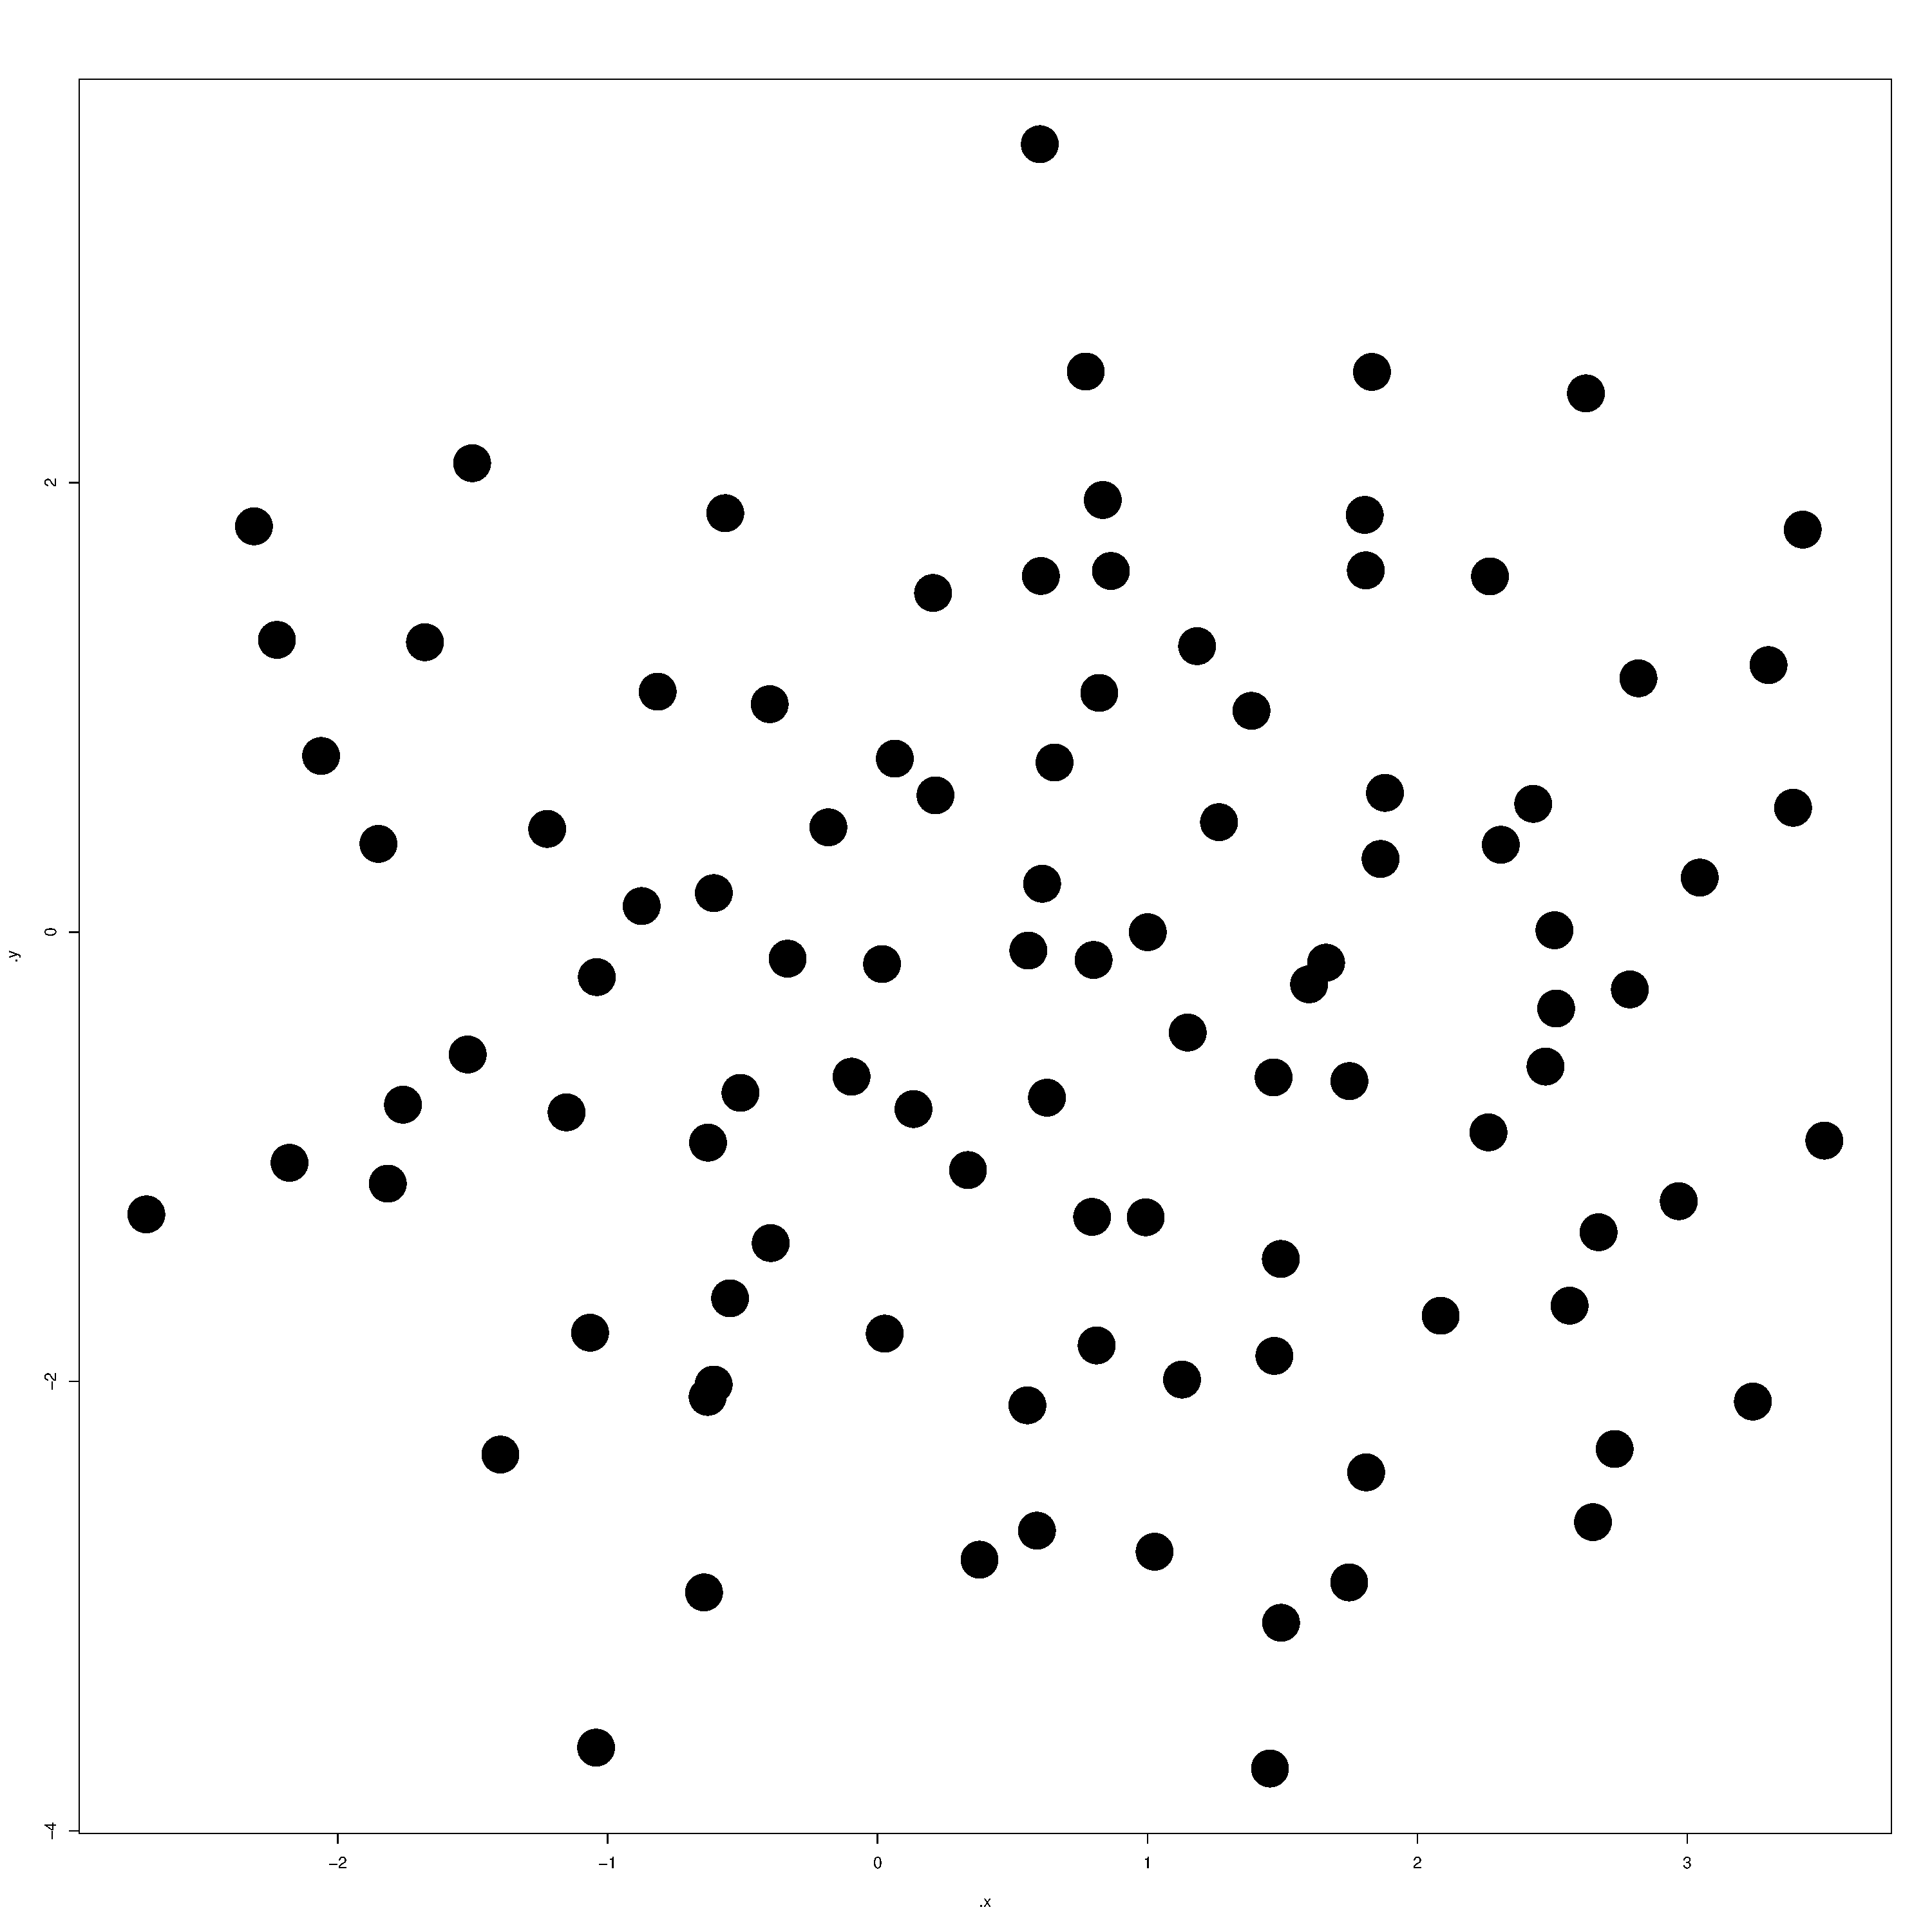
\includegraphics[height=2.5cm]{figures/blob_impl.pdf}
        \caption{No discernible clusters.}
    \end{subfigure}
    ~
    \begin{subfigure}[t]{0.45\textwidth}
	    \centering
        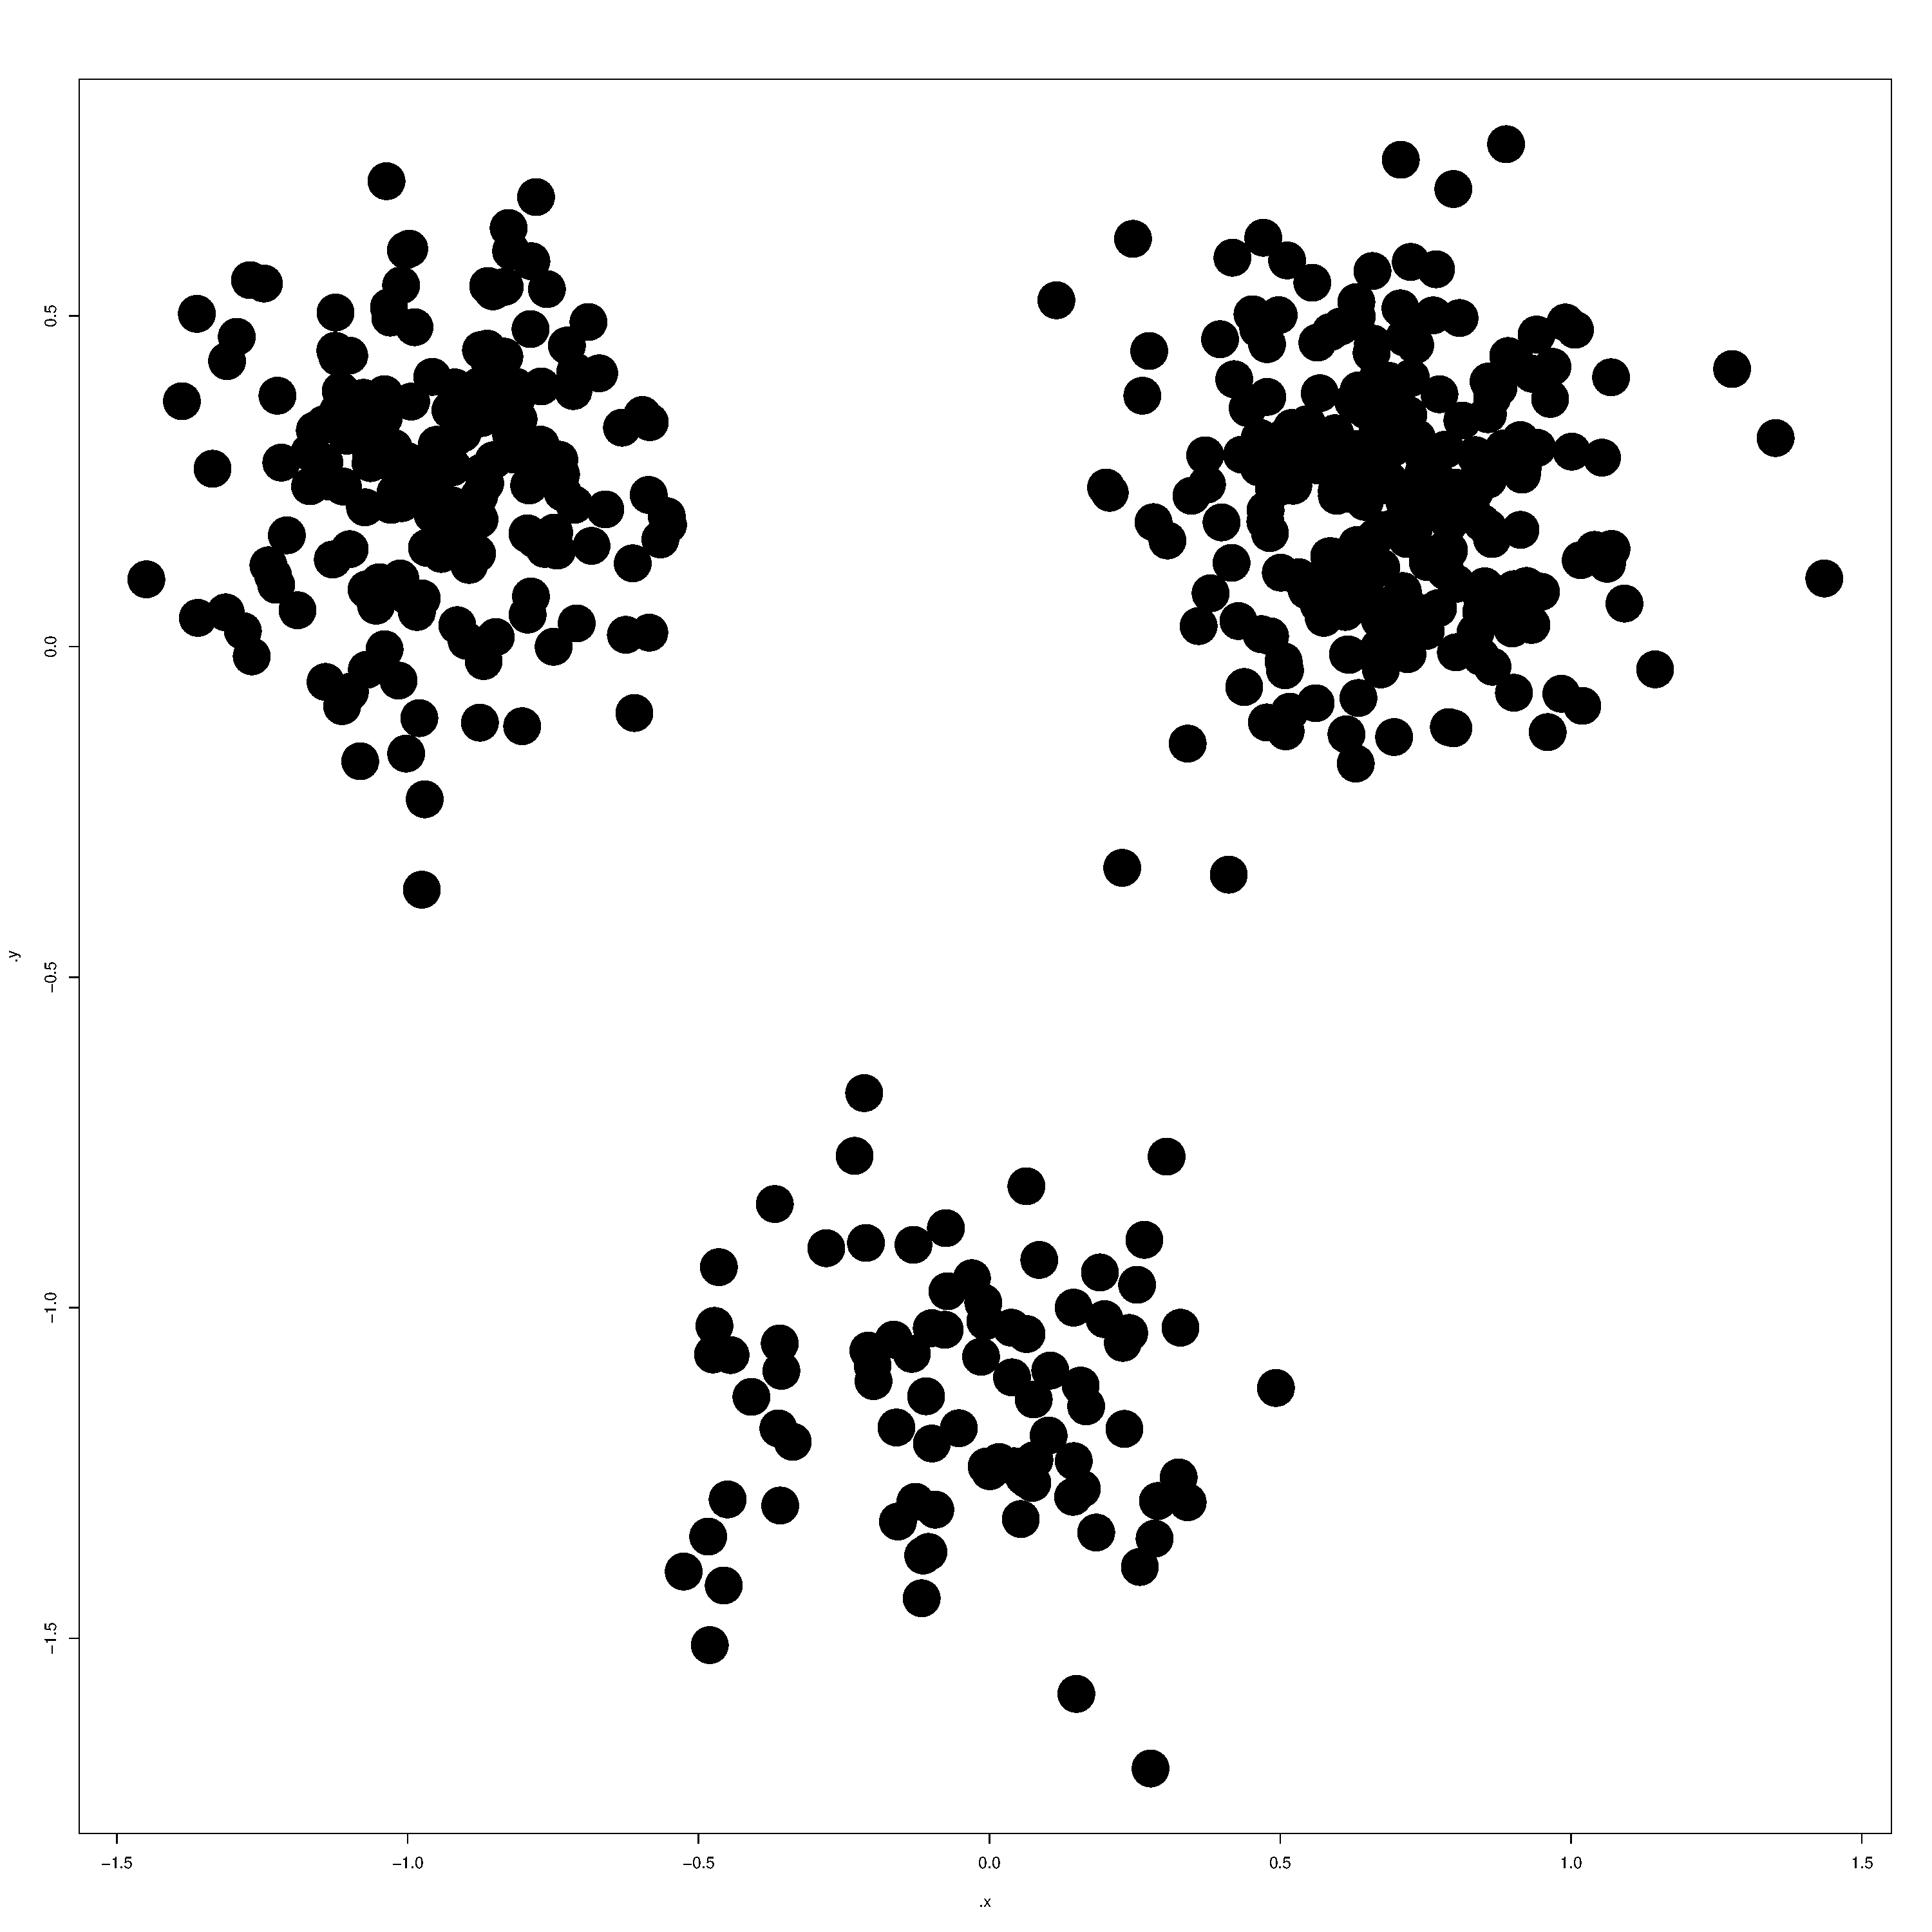
\includegraphics[height=2.5cm]{figures/clusters_impl.pdf}
        \caption{Three discernible clusters.}
    \end{subfigure}
    ~
    \begin{subfigure}[t]{0.45\textwidth}
	    \centering
        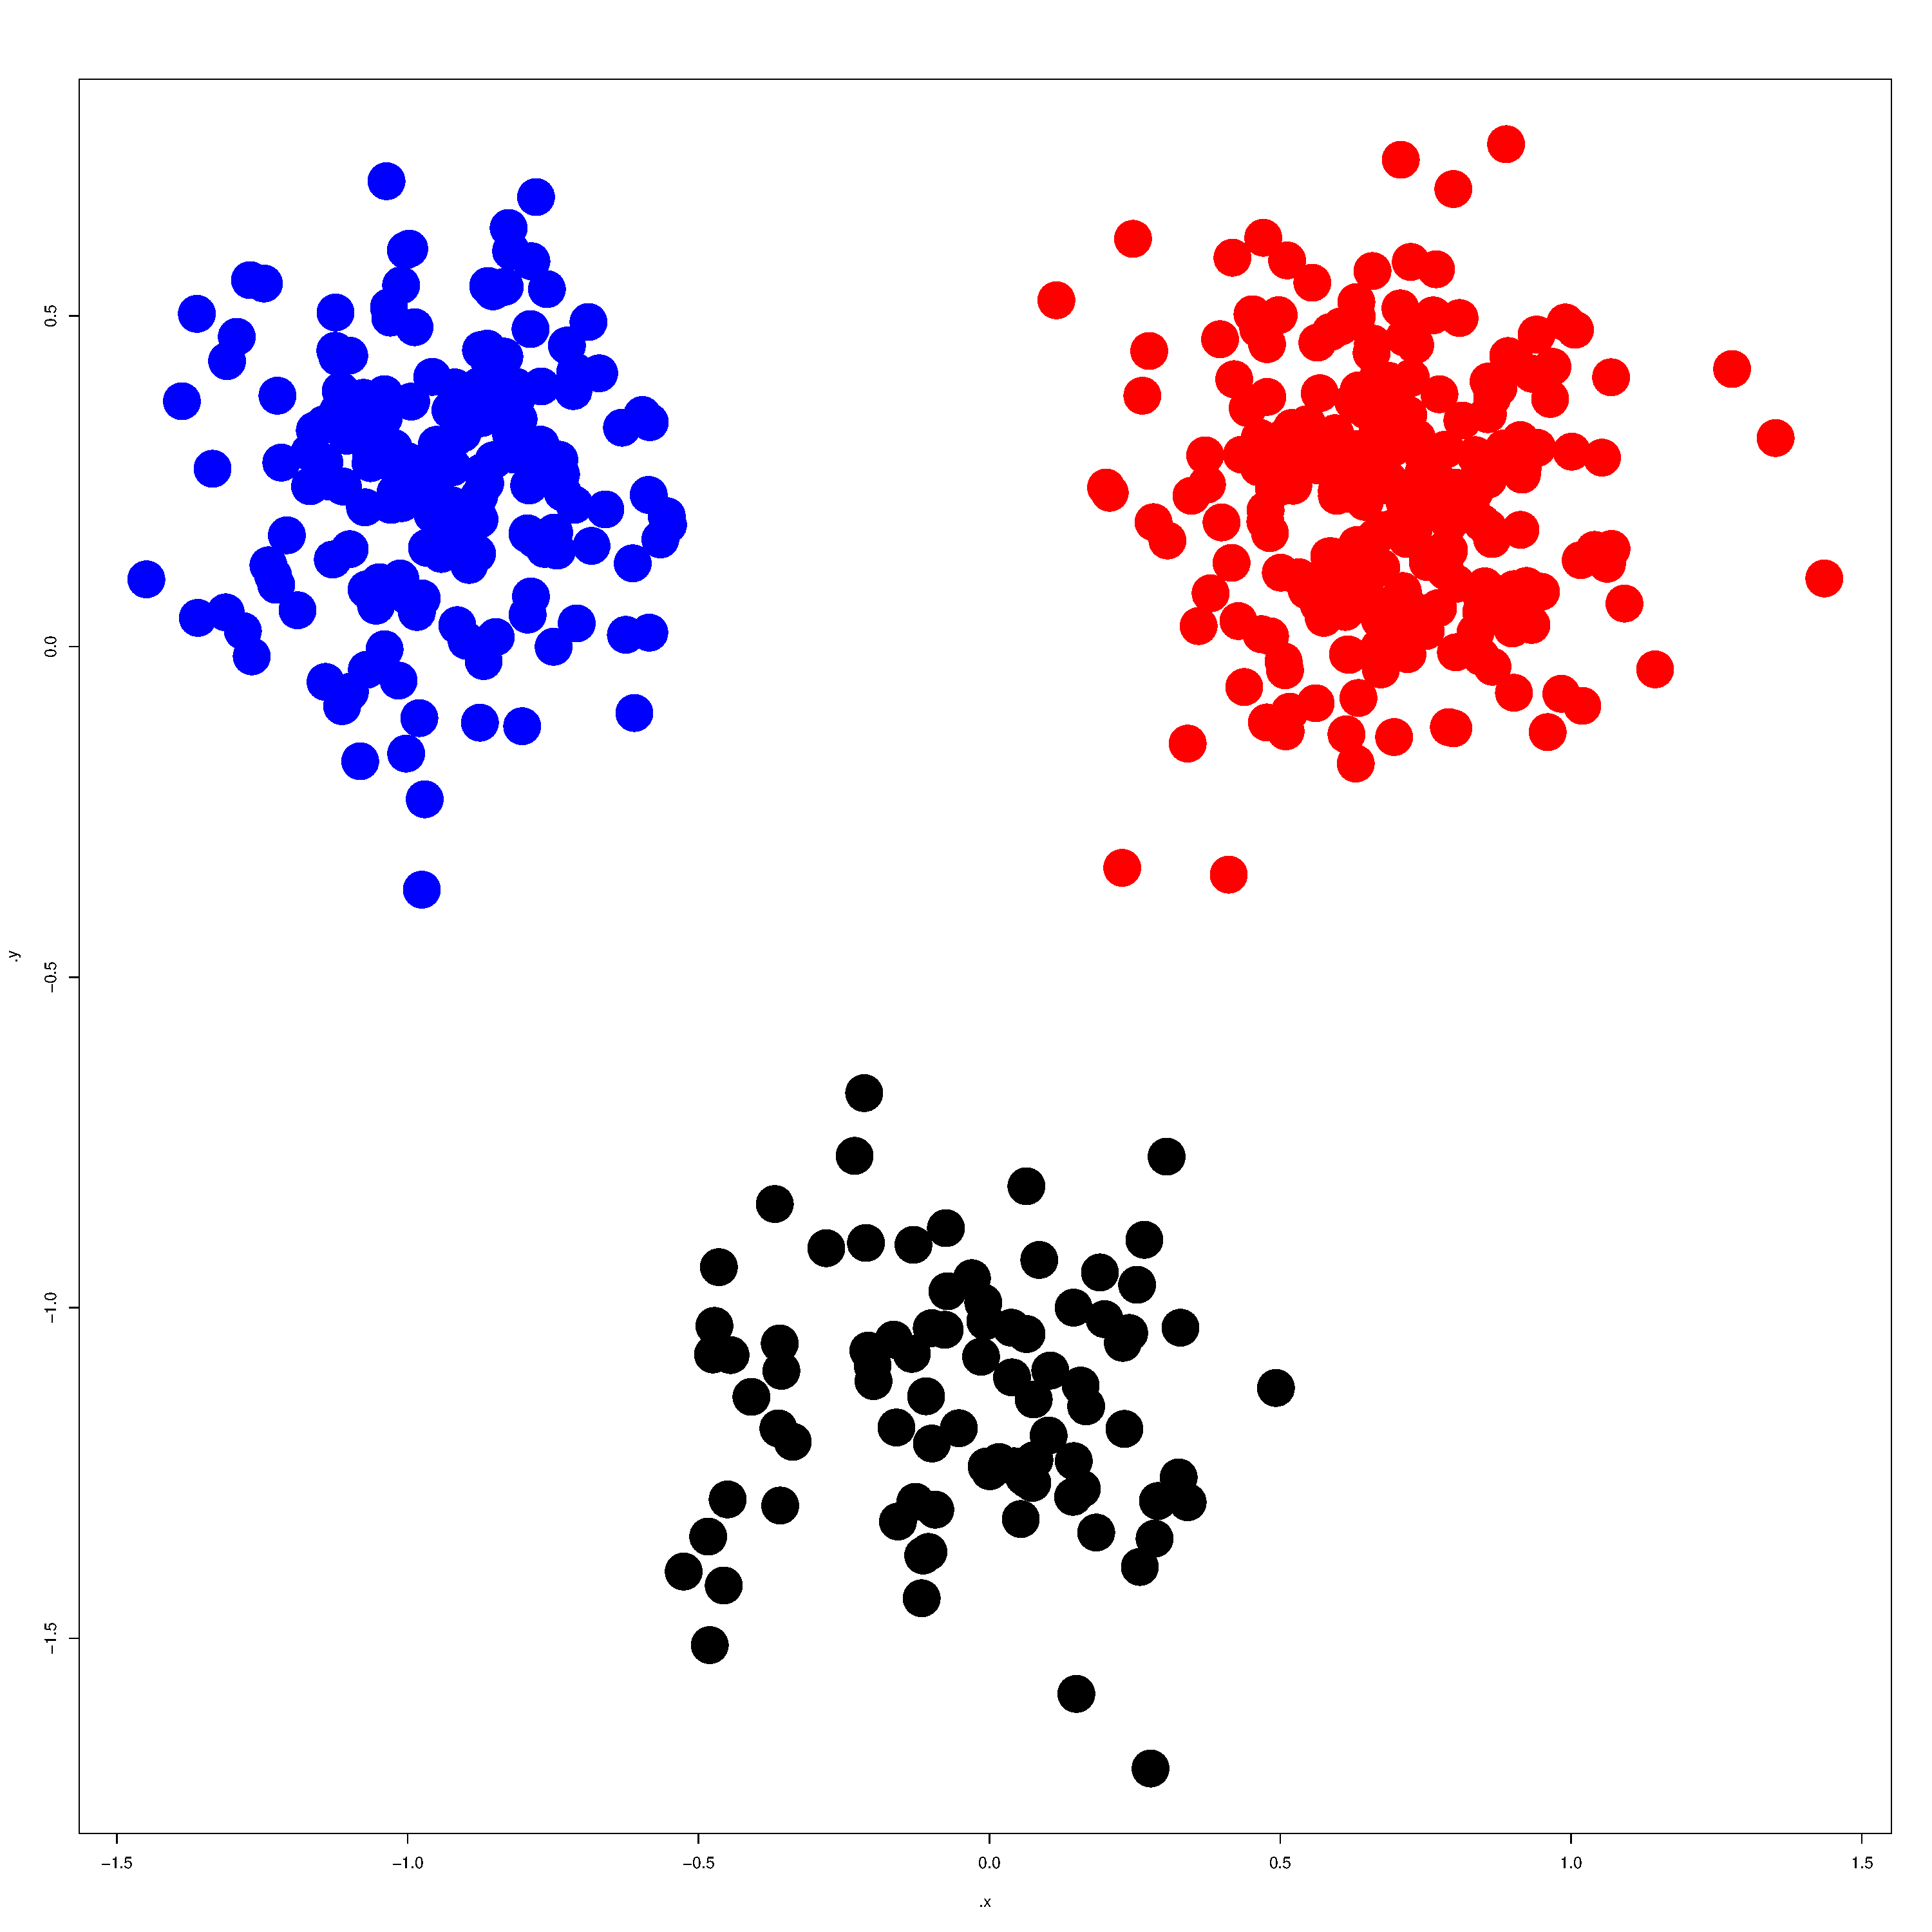
\includegraphics[height=2.5cm]{figures/clusters_expl.pdf}
        \caption{A match between clusters and class labels.}
    \end{subfigure}
    ~
    \begin{subfigure}[t]{0.45\textwidth}
	    \centering
        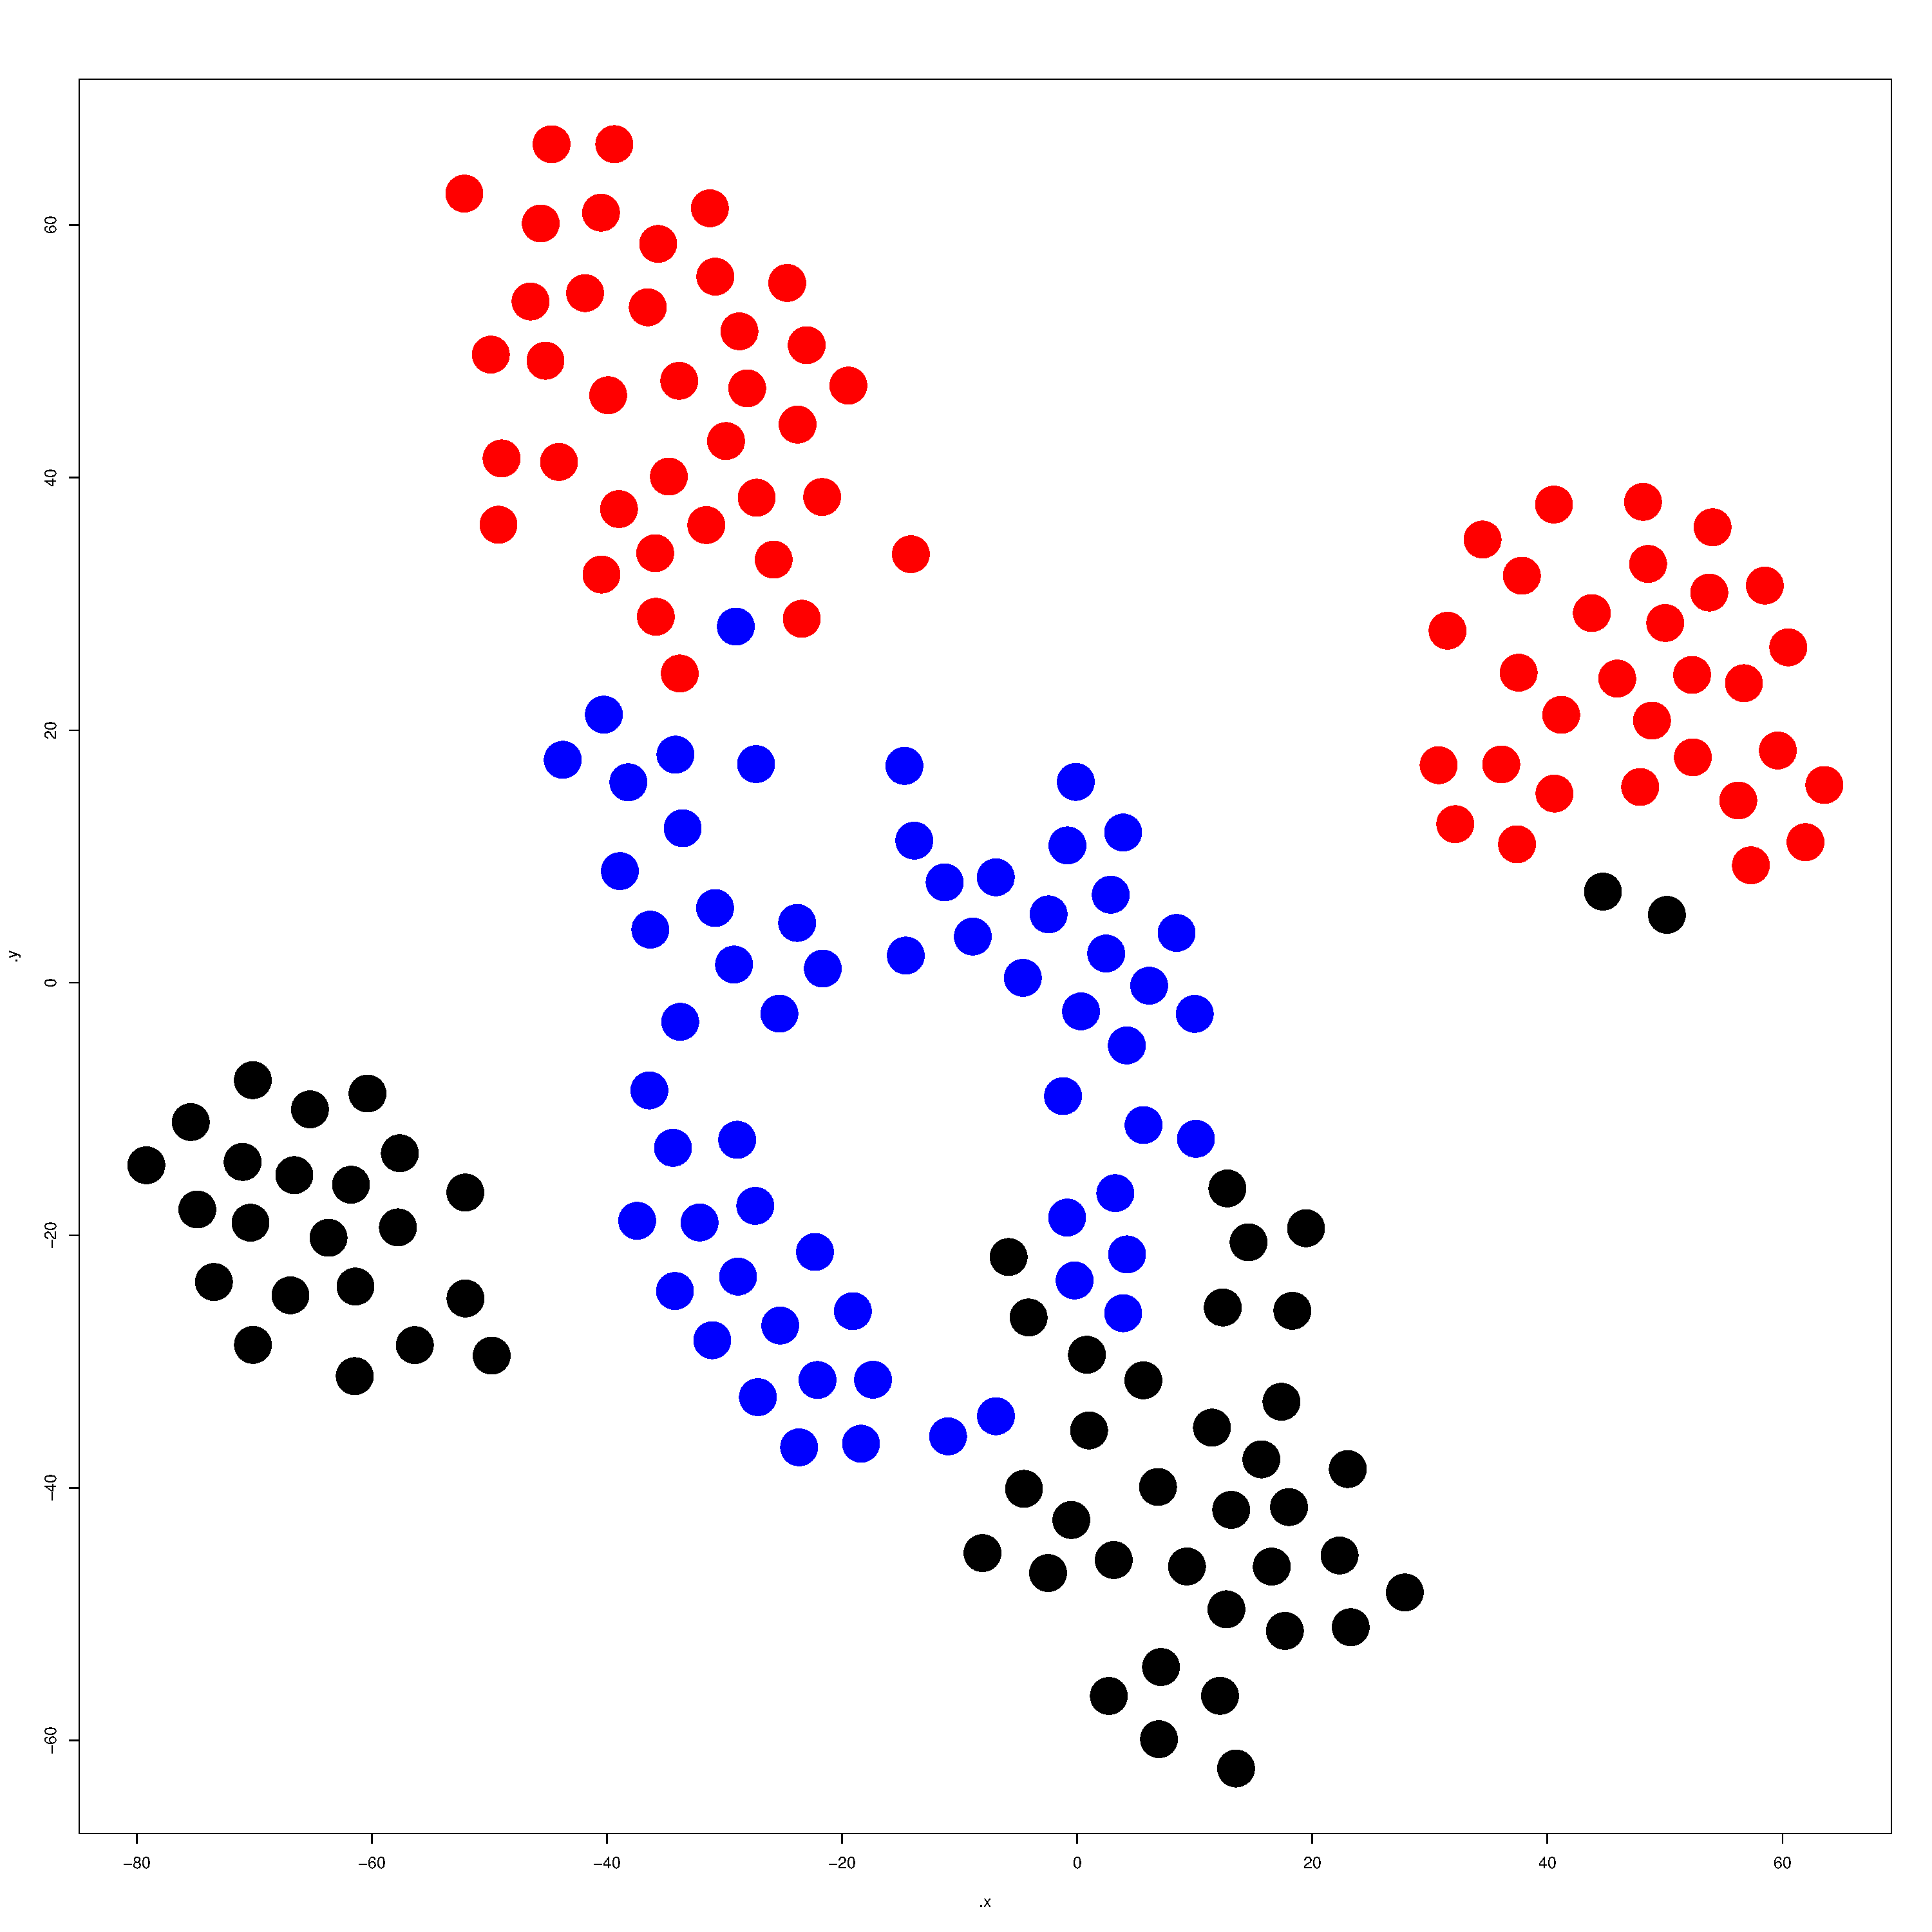
\includegraphics[height=2.5cm]{figures/clusters_expl_mismatch.pdf}
        \caption{A partial match between clusters and class labels.}
    \end{subfigure}
    ~
    \begin{subfigure}[t]{0.45\textwidth}
	    \centering
        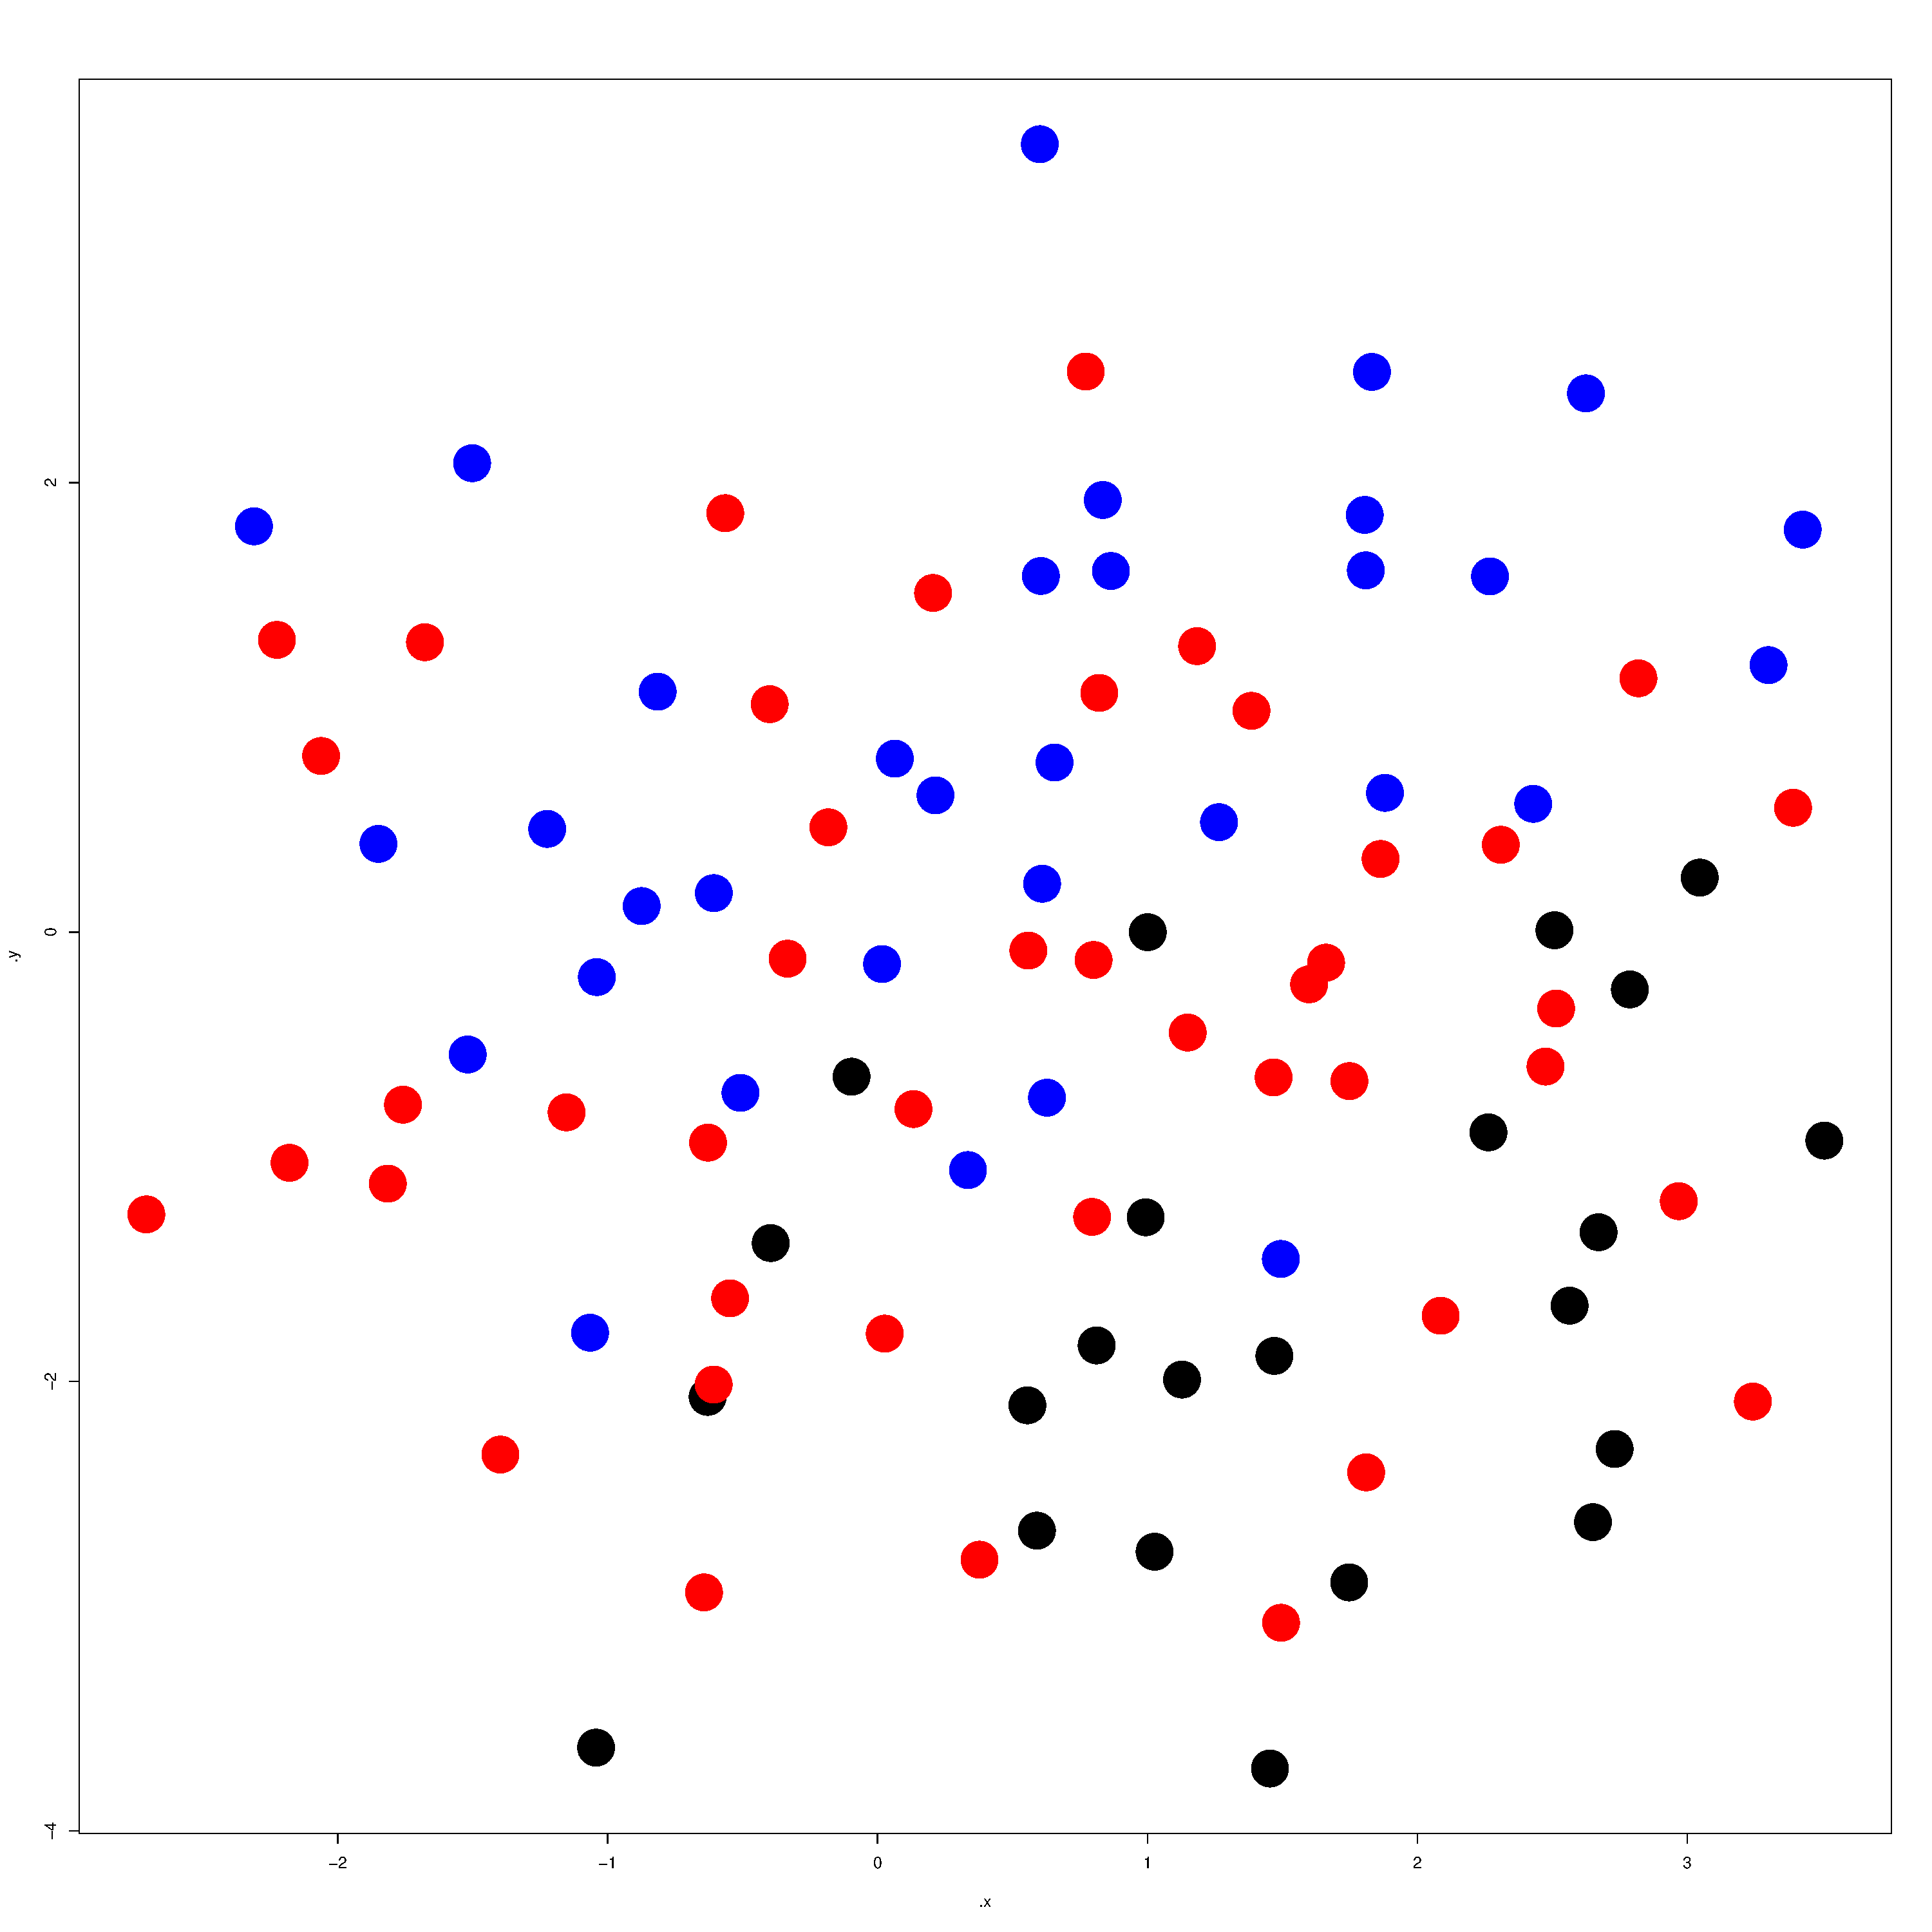
\includegraphics[height=2.5cm]{figures/blob_expl.pdf}
        \caption{No discernible class separation.}
    \end{subfigure}
	\caption
	[
	    Scatterplots of dimensionally reduced data illustrating tasks related to item clusters.
	]
	{
    	Example scatterplots of dimensionally reduced data illustrating tasks related to item clusters: Verifying the existence of clusters, naming clusters, and matching clusters and classes.
	}
	\centering
	\label{drvistasks:fig:clusters}
\end{figure}

%-|-|-|-|-|-|-|-|-|-|-|-|-|-|-|-|-|-|-|-|-|-|-|-|-|-|-|-|-|-|-|-|-|-|-|-|-

% %-------------------------------------------------------------------------

% \subsubsection{Verify Clusters}
% \label{drvistasks:tasks:verify-clusters}

%-------------------------------------------------------------------------

% \begin{figure}[!ht]
% 	\centering
% 	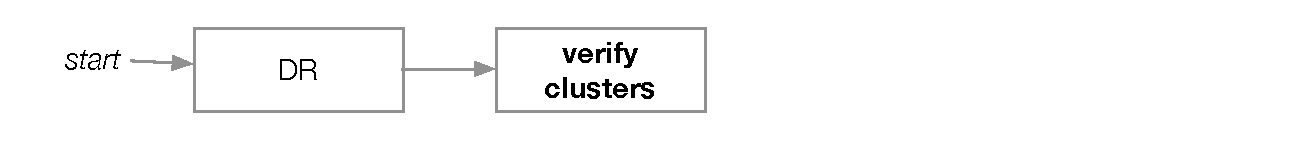
\includegraphics[width=\textwidth]{figures/drviztasks-identify-clusters.eps}
% 	\centering
% \end{figure}

\bstart{Verify clusters}
Analysts might seek to {\tt verify}\index{{\tt discover}} the hypothesis that clusters of items will be revealed in the dimensionally reduced\index{dimensionality reduction (DR)} data, or to {\tt verify}\index{{\tt discover}} hypotheses about specific conjectured clusters.
In order to {\tt discover}\index{{\tt discover}} clusters, analysts must {\tt locate}\index{{\tt locate}} and {\tt identify}\index{{\tt identify}} item clusters in the low-dimensional representation of the data; in the example of \autoref{drvistasks:fig:clusters}b, we can {\tt identify}\index{{\tt identify}} three clusters.

All ten of the analysts we spoke to were interested in verifying that clusters exist in their data. 
This task sequence\index{task!task sequence} is also captured by a discussion by \citet{Buja2002} about visualizing data following multidimensional scaling. 
The analysts we interviewed used a variety of visualization techniques when performing this task sequence\index{task!task sequence}, including two-dimensional monochrome scatterplots\index{visual encoding!scatterplot}, such as those depicted in \autoref{drvistasks:fig:clusters}a-b, as well as three-dimensional scatterplots\index{visual encoding!scatterplot!3D scatterplot}, \ac{SPLOM}s\index{visual encoding!scatterplot!scatterplot matrix (SPLOM)}, dendrograms\index{visual encoding!tree}, heat maps\index{visual encoding!heat map}, and density plots\index{visual encoding!density plot}. 

% %-------------------------------------------------------------------------

% \subsubsection{Name Clusters}
% \label{drvistasks:tasks:name-clusters}

% %-------------------------------------------------------------------------

% \begin{figure}[!ht]
% 	\centering
% 	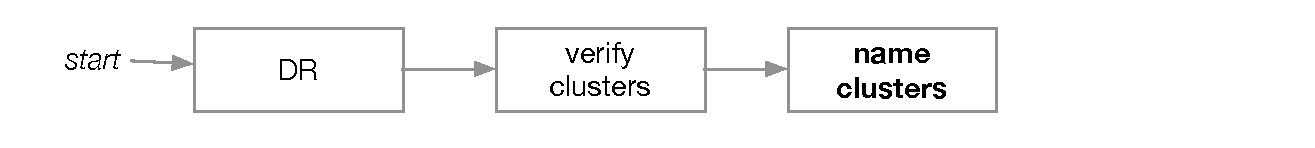
\includegraphics[width=\textwidth]{figures/drviztasks-name-clusters.eps}
% 	\centering
% \end{figure}

\bstart{Name clusters}
Once the existence of clusters has been verified, such as in the example of \autoref{drvistasks:fig:clusters}b, the next task\index{task} is often one of {\tt generating} hypotheses regarding the meaning of these clusters in the form of a name.
In this {\tt discover}\index{{\tt discover}} task\index{task}, an analyst will {\tt browse}\index{{\tt browse}} items within a cluster and attempt to {\tt summarize}\index{{\tt summarize}} the cluster with a meaningful name. 
In some cases, this name is made explicit, as the analyst will {\tt annotate}\index{{\tt annotate}} the cluster, thereby using the visual encoding\index{visual encoding} to {\tt produce}\index{{\tt produce}} new information about their data. 

Eight of the analysts who had previously {\it verified clusters} also attempted to {\it name clusters} in the course of their work, using the same visualization techniques. 
For instance,~\ref{drvistasks:analyst:HY} examined bibliometric data from a corpus of life sciences research literature, who attempted to {\tt identify}\index{{\tt identify}} and name clusters of related research concepts, such as {\it ``cancer''} or {\it ``RNA''}.

% %-------------------------------------------------------------------------

% \subsubsection{Match Clusters and Classes}
% \label{drvistasks:tasks:match-clusters}

% %-------------------------------------------------------------------------

% \begin{figure}[!ht]
% 	\centering
% 	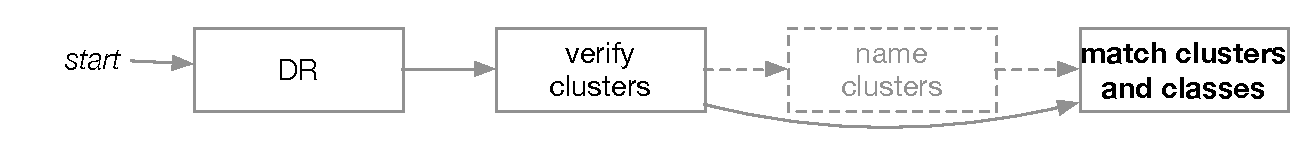
\includegraphics[width=\textwidth]{figures/drviztasks-match-clusters.eps}
% 	\centering
% \end{figure}

\bstart{Match clusters and classes}
The final task sequence\index{task!task sequence} we characterize is matching clusters with classes. 
The {\tt input}\index{{\tt input}} to this {\it match} task\index{task} is not only a set of item clusters, {\tt identified}\index{{\tt identify}} in the earlier {\it verify clusters} task\index{task}, but also a set of categorical class labels.
These classes might come directly with the data, be assigned using a clustering algorithm\index{algorithms!clustering} run by the analyst, or be the result of manual labeling. 
The analyst must {\tt verify}\index{{\tt discover}} a hypothesis that a cluster of items matches the class for those items. 
To {\tt discover}\index{{\tt discover}} a match, the analyst performs a {\tt lookup}\index{{\tt lookup}} for the class and cluster membership of an item in order to {\tt compare}\index{{\tt compare}} them, resulting in a match (as in \autoref{drvistasks:fig:clusters}c), otherwise referred to as a {\it true positive}, or a mismatch (as in \autoref{drvistasks:fig:clusters}d-e), which could either be a {\it true negative} or a {\it false negative}.
This task\index{task} was examined in our recent paper~\cite{Sedlmair2013}, a paper that offered guidance for choosing appropriate visualization techniques for dimensionally reduced\index{dimensionality reduction (DR)} data.

Naming the clusters is not a pre-requisite for this {\it match} task\index{task}, though we did encounter four analysts who reported performing both tasks\index{task} in succession (\ref{drvistasks:analyst:JB}, \ref{drvistasks:analyst:HL}, \ref{drvistasks:analyst:DH}, \ref{drvistasks:analyst:JS}); two other analysts performed this task\index{task} without previously naming the clusters they identified\index{{\tt identify}} (\ref{drvistasks:analyst:KA}, \ref{drvistasks:analyst:AC}).
Typically, this task\index{task} was performed using two-dimensional scatterplots\index{visual encoding!scatterplot}, wherein the points were coloured using the class labels; \ac{SPLOM}s\index{visual encoding!scatterplot!scatterplot matrix (SPLOM)}, interactive and non-interactive three-dimensional scatterplots\index{visual encoding!scatterplot}, and node-link graphs were also used.
Note that the visual separability of colour-coded clusters differs perceptually from the separability of monochrome clusters, as described in our recent taxonomy of cluster separation factors~\cite{Sedlmair2012a}. 
These perceptual differences should be taken into account particularly when determining which experimental stimuli for use in controlled experiments.

A possible outcome of this task sequence\index{task!task sequence} is a partial match between classes and clusters: there may be more clusters than classes, or vice versa.
In cases where there are more clusters than class labels, illustrated in \autoref{drvistasks:fig:clusters}d, this outcome suggests that the class labels may not capture a finer-grained cluster structure in the data, as was the case for the investigative journalist\index{journalism} that we interviewed (\ref{drvistasks:analyst:JS}). 
In cases where there are more classes than clusters, illustrated in \autoref{drvistasks:fig:clusters}e, this result may either be a {\it true negative}, in which perfect class separation is not possible, or a {\it false positive}~\cite{Sedlmair2013}.
If this mismatch is suspected to be a {\it false negative}, Sedlmair~\etal~recommend {\tt selecting}\index{{\tt select}} other dimensions to visualize, using other design choices such as a \ac{SPLOM}\index{visual encoding!scatterplot!scatterplot matrix (SPLOM)}, or revisiting the choice of \ac{DR}\index{dimensionality reduction (DR)} technique. 

%-------------------------------------------------------------------------
%-------------------------------------------------------------------------

\section{A Task Typology Revisited}
\label{drvistasks:typology}

%-------------------------------------------------------------------------
%-------------------------------------------------------------------------

The analysts that we interviewed hailed from very different domains, each using a different terminology to describe their work processes\index{work domain analysis}.
For instance, we needed a way to compare how {\it diagnosing cancer patients based on their genomic data} (\ref{drvistasks:analyst:AC}) was like {\it classifying types of human motion through the use of sensors attached to the body} (\ref{drvistasks:analyst:KA}).
We required an abstract vocabulary\index{task!task abstraction} for describing and comparing the work processes of these analysts.

For this reason, we used our typology\index{task!task typology} of abstract visualization tasks\index{task!task abstraction}, introduced in \autoref{ch:typology}, which provided a domain-agnostic vocabulary and framework for describing visualization tasks\index{task} in terms of {\it why}\index{{\tt why}}, {\it what}\index{{\tt what}}, and {\it how}\index{{\tt how}}.
By describing a task\index{task} in this manner, we can link {\tt outputs}\index{{\tt output}} and {\tt inputs}\index{{\tt input}} to describe sequences\index{task!task sequence} of interdependent tasks\index{task}, which Norman would refer to as {\it activities}~\cite{Norman2005}. 
% This typology has already been used to characterize the tasks of journalists~\cite{Brehmer2014}\footnote{This classification of journalists' tasks is documented in \autoref{ch:overview}.} and bioinformaticians~\cite{Mirel2014}. 
We use it here to describe task sequences\index{task!task sequence} relating to visualizing dimensionally reduced\index{dimensionality reduction (DR)} data across multiple domains.

Our analysis concentrated on the {\it why}\index{{\tt why}} and {\it what}\index{{\tt what}} aspects of the tasks\index{task} pertaining to dimensionally reduced\index{dimensionality reduction (DR)} data, as summarized in \autoref{drvistasks:fig:drviztasks}.
We chose not to be prescriptive about {\it how}\index{{\tt how}} these task sequences\index{task!task sequence} should best be supported by visualization techniques; instead, we described the variety of techniques used by the analysts that we interviewed for each task sequence\index{task!task sequence}, as summarized in \autoref{drvistasks:tab:summary}.

%-|-|-|-|-|-|-|-|-|-|-|-|-|-|-|-|-|-|-|-|-|-|-|-|-|-|-|-|-|-|-|-|-|-|-|-|-

\begin{figure}
	\centering
	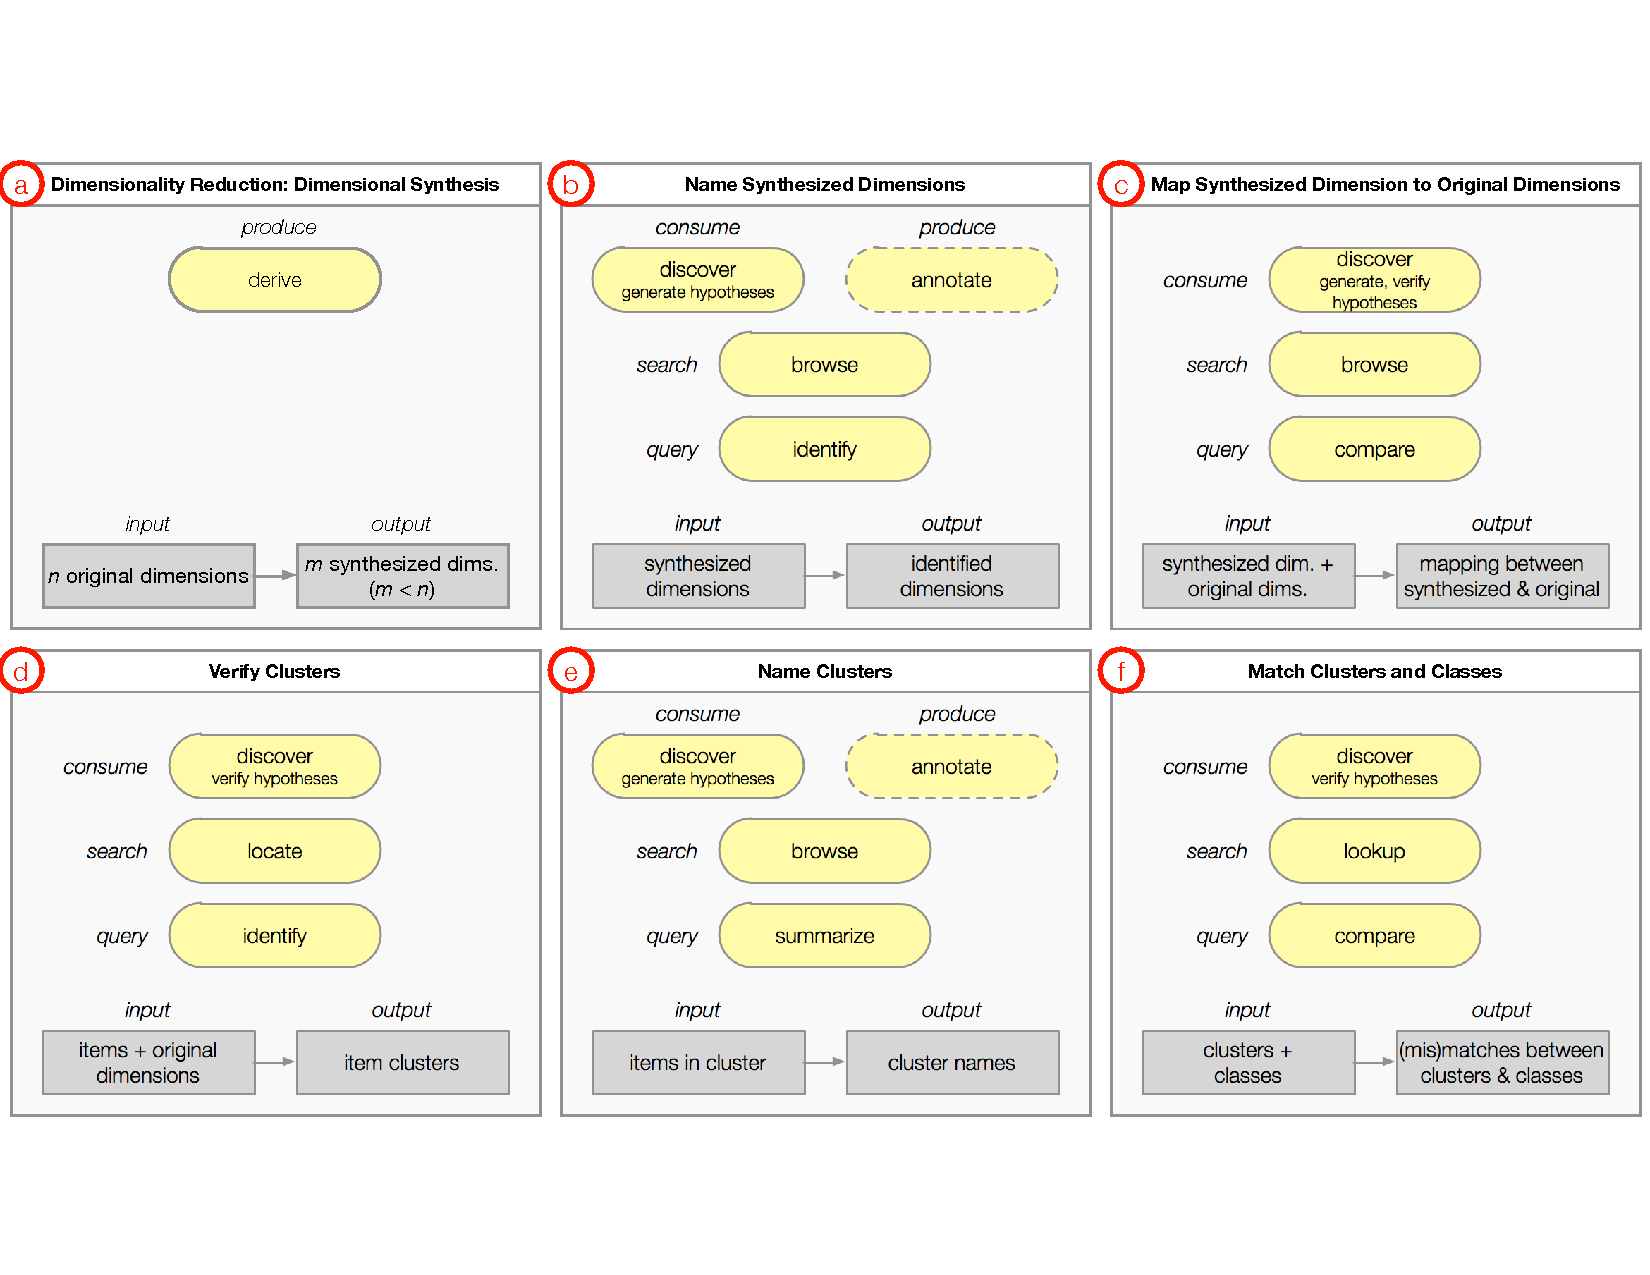
\includegraphics[width=\textwidth]{figures/drviztasks.pdf}
	\caption
	[
	    Six tasks related to dimensionally reduced data, characterized using our abstract task typology.
	]
	{
	    Six tasks related to dimensionally reduced data, characterized using our abstract task typology introduced in \autoref{ch:typology}, which describes \textsl{why} the data is being visualized at multiple levels of abstraction (yellow) and \textsl{what} {\tt inputs} and {\tt outputs} a task has (grey). These tasks are combined to form the task sequences described in \autoref{drvistasks:tasks}.
	}
	\centering
	\label{drvistasks:fig:drviztasks}
\end{figure}

%-|-|-|-|-|-|-|-|-|-|-|-|-|-|-|-|-|-|-|-|-|-|-|-|-|-|-|-|-|-|-|-|-|-|-|-|-

The analysts we interviewed were all interested in {\tt discovery}, which involves the {\tt generation} and {\tt verification} of hypotheses. 
\autoref{drvistasks:fig:drviztasks}b-f show which tasks\index{task} relate to {\tt hypothesis generation}\index{{\tt discover}} and which relate to {\tt hypothesis verification}\index{{\tt discover}}. 
The graphical depiction also shows which task\index{task} can be associated with pure {\tt consumption} of information and which task\index{task} can additionally lead to the {\tt production} of new information.
When consuming information, an analyst will {\tt search}\index{{\tt search}} for targets within a visual encoding\index{visual encoding}.
Whether the location and identity of these targets is known a priori will determine the type of {\tt search}\index{{\tt search}}. 
In tasks\index{task} related to visualizing dimensionally reduced\index{dimensionality reduction (DR)} data, we found that {\tt search}\index{{\tt search}} strategies used by analysts were either {\tt browse}\index{{\tt browse}}, {\tt locate}\index{{\tt locate}}, or {\tt lookup}\index{{\tt lookup}}, as indicated in \autoref{drvistasks:fig:drviztasks}b-f. 
Once targets are found, an analyst will execute some form of {\tt query}\index{{\tt query}}: they might {\tt identify}\index{{\tt identify}} a single target, such as an item cluster, {\tt compare}\index{{\tt compare}} multiple targets, such as values along a synthesized dimension to values along an original dimension, or {\tt summarize}\index{{\tt summarize}} all the targets, such as when {\it naming a cluster}. 

\bstart{Dependencies} 
The task sequences\index{task!task sequence} described in \autoref{drvistasks:tasks} contain dependencies. 
For example, in order to {\it match clusters and classes}, an analyst must first {\it verify}\index{{\tt discover}} that clusters exist. 
Each of the sequences\index{task!task sequence} also depend on the {\tt output}\index{{\tt output}} of \ac{DR}\index{dimensionality reduction (DR)} techniques, the {\tt derived}\index{{\tt derive}} synthetic dimensions.  
The application of \ac{DR}\index{dimensionality reduction (DR)} to a set of original dimensions is itself a task\index{task}, as shown in \autoref{drvistasks:fig:drviztasks}a. 
However, unlike the other tasks\index{task} described in this chapter, it is about neither hypothesis generation nor verification, but rather about {\tt producing}\index{{\tt produce}} new information intended to support subsequent tasks\index{task}.

While the distinctions between these tasks\index{task} and task sequences\index{task!task sequence} may seem obvious in hindsight, we initially struggled to find a vocabulary and framework that would allow us to distinguish between these task sequences\index{task!task sequence} and their interdependencies.
Our task typology\index{task!task typology}, introduced in \autoref{ch:typology}, allows us to describe these task sequences\index{task!task sequence} explicitly, whereas they were implicit in previous work combining \ac{DR}\index{dimensionality reduction (DR)} and visualization.

\bstart{Extended typology}
\autoref{drvistasks:fig:typology} reproduces the {\it why}\index{{\tt why}} part of an extended task typology~\cite{Munzner2014}\footnote{We comment further on the the extensions to our typology in \autoref{conclusions:typology:extension}.}.

%-|-|-|-|-|-|-|-|-|-|-|-|-|-|-|-|-|-|-|-|-|-|-|-|-|-|-|-|-|-|-|-|-|-|-|-|-

\begin{figure}
	\centering
	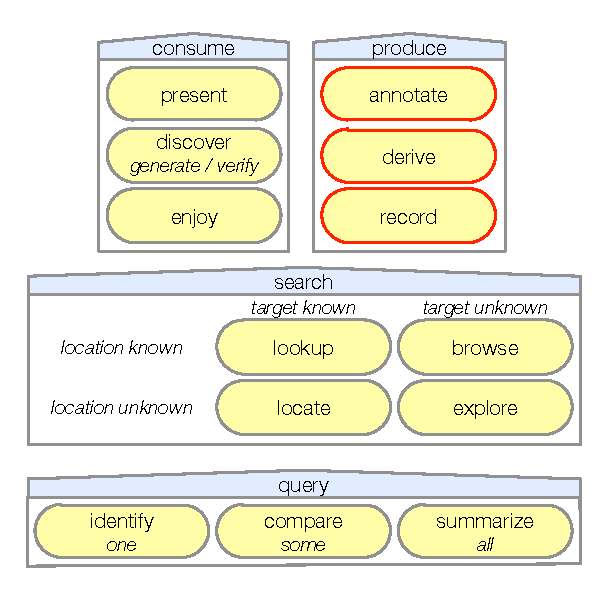
\includegraphics[width=0.7\textwidth]{figures/typology-why.eps}
	\caption
	[
	    A refinement to the \textsl{why} part of our abstract task typology.
	]
	{
    	The \textsl{why} part of our abstract task typology from \autoref{ch:typology}, with the refinement (emphasized in red) that the actions of {\tt annotate}, {\tt record}, and {\tt derive} are forms of {\tt produce}~\cite{Munzner2014}.
    }
    \centering
	\label{drvistasks:fig:typology}
\end{figure} 

%-|-|-|-|-|-|-|-|-|-|-|-|-|-|-|-|-|-|-|-|-|-|-|-|-|-|-|-|-|-|-|-|-|-|-|-|-

The changes relevant to our analysis in this chapter pertain to three actions: an analyst may {\tt annotate}\index{{\tt annotate}} information, {\tt derive}\index{{\tt derive}} new information from existing, or {\tt record}\index{{\tt record}} their use of a visualization tool so as to provide analytical provenance or to facilitate subsequent presentations of the visualized data. 
The terms {\tt annotate}\index{{\tt annotate}}, {\tt derive}\index{{\tt derive}}, and {\tt record}\index{{\tt record}} were previously attributed to families of interaction\index{interaction} design choices in the {\it how}\index{{\tt how}} part of our typology\index{task!task typology}; the extended typology\index{task!task typology} classifies them as ends\index{task!ends} rather than means\index{task!means} and thus situates them as forms of {\tt produce}\index{{\tt produce}}.
Both versions of the typology\index{task!task typology} distinguish whether a person will visualize data either to {\tt consume}\index{{\tt consume}} or {\tt produce}\index{{\tt produce}} information. 
The remaining aspects of the typology\index{task!task typology} describing lower levels of abstraction\index{task!task abstraction} are unchanged. 

%-------------------------------------------------------------------------
%-------------------------------------------------------------------------

\section{Discussion}
\label{drvistasks:discussion}

%-------------------------------------------------------------------------
%-------------------------------------------------------------------------

We discuss the utility of our classification of task sequences\index{task!task sequence} with regard to several visualization evaluation\index{evaluation} scenarios, the limitations of our current findings, and our planned future work.

%-------------------------------------------------------------------------

\subsection{Implications for Evaluation}
\label{drvistasks:discussion:evaluation}

%-------------------------------------------------------------------------

Task analysis\index{task!task analysis} and evaluation\index{evaluation} are closely linked. 
An understanding of visualization tasks\index{task} informs how an evaluation\index{evaluation} is conducted, from the justification of experimental procedures to the collection and analysis of field observations.

Our current work adds to previous task\index{task} classifications proposed in the visualization evaluation\index{evaluation} literature~\cite{Henry2006,Lee2006,Valiati2006}.
As evaluation\index{evaluation} takes on many forms, we frame our discussion around four of Lam~\etal's scenarios for empirical studies~\cite{Lam2012}.

\bstart{Understanding work practices}
Work practice evaluation\index{evaluation} or work domain analysis\index{work domain analysis} can provide a richer understanding of the perspective of people who might benefit from visualizing their data, reflecting real work practices and activities.
While we have outlined their immense importance several times~\cite{Brehmer2014a,Meyer2015,Munzner2009}, only a few dedicated examples exist in the visualization literature~\cite{Kandel2012,Kang2011,Tory2008}.

More commonly, however, such work practice evaluations\index{evaluation} occur in design studies\index{design studies}, an increasingly popular form of problem-driven visualization research.
In particular, a design study's early {\it discover stage}~\cite{Sedlmair2012} involves the analysis of work practices\index{work domain analysis} within a very specific usage context in a particular domain.
These concrete work practices are then translated into abstract visualization tasks\index{task!task abstraction} and design requirements.

Our current work goes beyond task\index{task} classification in design studies\index{design studies} by conducting interviews with analysts across different application domains. 
We then cast our findings as task sequences\index{task!task sequence} or activities~\cite{Norman2005} that abstract away domain-specific language.
In doing so, we intend to support researchers when conducting and analyzing future {\it work practice} evaluations\index{evaluation}, 
specifically when \ac{DR} techniques are to be used. 
We encourage practitioners to adopt our classification of task sequences\index{task!task sequence} into a lexicon for coding observations\index{coding (qualitative data analysis)} of work practices and for translating domain-specific descriptions of these practices.
We believe that using our task sequences\index{task!task sequence} will make the analysis process more efficient and, furthermore, will allow for transferability between design studies\index{design studies} from different application domains~\cite{Sedlmair2012}.

\bstart{Evaluating human performance}
Our classification of task sequences\index{task!task sequence} can inform the design of experimental procedures and participant instructions in controlled laboratory studies, where the aim might be to quantitatively assess human performance on a newly proposed visualization technique.
Many previous classifications of tasks have informed experimental design, such as the adoption of a task classification by \citet{Zhou1998} in a laboratory evaluation\index{evaluation} of an information retrieval\index{information retrieval} tool~\cite{Morse2000}.
We expect that our classification of task sequences\index{task!task sequence} will play a similar role in the evaluation\index{evaluation} of techniques or tools that visualize dimensionally reduced\index{dimensionality reduction (DR)} data. 
For instance, an experiment might compare multiple visualization techniques for {\it verifying clusters} and subsequently {\it matching clusters and classes}, where performance might be measured in terms of speed and accuracy.

\citet{Munzner2009} refers to such studies as a form of downstream validation, in which a design has been implemented for its investigation in a study. 
In contrast, upstream validation in this case refers to the justification of visual encoding\index{visual encoding} and interaction\index{interaction} design choices before its implementation. 
We deem our task sequences\index{task!task sequence} to be similarly helpful for such upstream evaluations\index{evaluation}. 
Researchers presenting new visual encoding\index{visual encoding} or interaction\index{interaction} design choices can refer to our task sequences\index{task!task sequence} to concisely state assumptions about which abstract tasks\index{task!task abstraction} are supported, rather than leaving this description implicit in a way that places a burden on a potential adopter\index{adoption} of the design choice. 

\bstart{Evaluating the experience of using a visualization tool or technique}
In either lab or field settings, a researcher can evaluate\index{evaluation} the experience of using a tool or technique by dictating the tasks\index{task} without specifying {\it how}\index{{\tt how}} to execute them, asking study participants to verbalize their actions while they attempt to execute a sequence of tasks\index{task!task sequence}. 
Such a think-aloud protocol\index{evaluation!think-aloud evaluation} might allow the researcher to understand if features of the tool are learnable, useful, or in need of further usability improvements.
Questionnaires and interview questions relating to the experience of using a visualization tool or technique could also be framed around our classification of task sequences\index{task!task sequence}.

We note that expertise has many facets; the distinction between novices and experts is a particularly nuanced question for studies considering \ac{DR}\index{dimensionality reduction (DR)}.
Several of the high-dimensional data\index{high-dimensional data} analysts that we interviewed might be described as {\it middle-ground users}~\cite{Ingram2010}: they had significant domain expertise but only a partial understanding of the available \ac{DR}\index{dimensionality reduction (DR)} tools and of the mathematics underlying these techniques. 
This characteristic is important to keep in mind when recruiting participants for evaluations\index{evaluation} of performance or experience, as some evidence exists that participants with an understanding of \ac{DR}\index{dimensionality reduction (DR)} will interpret visual encodings\index{visual encoding} of dimensionally reduced\index{dimensionality reduction (DR)} data differently than those who do not have this understanding~\cite{Lewis2012}. 

\bstart{Evaluating visual data analysis and reasoning}
While a researcher must dictate the tasks\index{task} in a controlled laboratory experiment, another scenario is the observation of tasks\index{task} in an open-ended qualitative evaluation\index{evaluation} of a visualization tool or technique.
Here, the researcher must recognize when these task sequences\index{task!task sequence} appear in naturalistic settings, in order to better understand how visual data analysis and reasoning are supported following the introduction of a new visualization tool.
This form of evaluation\index{evaluation} is typical in design studies~\cite{Sedlmair2012,Shneiderman2006}\index{design studies}, particularly after a tool is deployed.

As with evaluations\index{evaluation} of work practices\index{work domain analysis}, our classification of task sequences\index{task!task sequence} could become part of a lexicon for coding\index{coding (qualitative data analysis)} observed behaviour after a tool is deployed.
In cases where direct observation of tool use is not possible, our classification of task sequences\index{task!task sequence} might be used to analyze interaction log\index{interaction!interaction logs} files, or used as a basis for diary or interview questions, suggesting a consistent vocabulary for coding\index{coding (qualitative data analysis)} participant responses. 
Precedents for the use of task\index{task} classification in evaluation\index{evaluation} of deployed tools include the adoption of a classification by \citet{Yi2007} in a longitudinal field study of a social network\index{social networks} analysis tool~\cite{Perer2009}, or how we used our task typology introduced in \autoref{ch:typology}\index{task!task typology} to evaluate\index{evaluation} why and how journalists\index{journalism} used {\it Overview}\index{Overview (document mining tool)}, a tool for analyzing large document collections~\cite{Brehmer2014}\footnote{This use of the task typology is documented in \autoref{ch:overview}.}.

Finally, if we consider the task sequences {\it name synthesized dimensions} and {\it name clusters} in particular, one conceivable evaluation\index{evaluation} of visual data analysis and reasoning would involve collecting participant annotations\index{{\tt annotate}} and explanations of synthesized dimensions or clusters in visual encodings\index{visual encoding} of dimensionally reduced\index{dimensionality reduction (DR)} data.
Such a study might adopt a protocol similar to one used by \citet{Willett2012} to elicit participant annotations\index{{\tt annotate}} and explanations of visualized time series data in an application deployed online.
This evaluation\index{evaluation} could help to identify the features of a visualization tool that facilitate or inhibit visual data analysis and reasoning.

%-------------------------------------------------------------------------

\subsection{Limitations}
\label{drvistasks:discussion:limitations}

%-------------------------------------------------------------------------

Our interview findings are certainly not exhaustive, and despite conducting interviews with nineteen analysts, only ten of these analysts contributed to our classification of task sequences\index{task!task sequence}. 
This selection was based on our goal of studying task sequences\index{task!task sequence} relating to visualizing data reduced with {\it dimensional synthesis}\index{dimensionality reduction (DR)!dimensional synthesis} techniques.
There are many other interesting areas of high-dimensional data\index{high-dimensional data} analysis that we did not address. 
Specifically, we found that many of our excluded interviewees used {\it dimensional filtering}\index{dimensionality reduction (DR)!dimensional filtering} techniques, in which a subset of the original dimensions are retained~\cite{Johansson2009,Yang2003}. 
Alternatively, other analysts applied \ac{DR}\index{dimensionality reduction (DR)} to their data without visually analyzing it. 
In these cases, \ac{DR}\index{dimensionality reduction (DR)} was used to reduce the data for algorithmic input\index{algorithms!algorithmic input}, such as for classification\index{algorithms!classification} and other machine learning\index{machine learning} applications. 

We consider our findings to be existence proofs of the task sequences\index{task!task sequence} as performed by analysts as part of their ongoing work. 
We do not make claims about the prevalence of these task sequences\index{task!task sequence} in high-dimensional data\index{high-dimensional data} analysis, nor do we make claims about completeness: our classification of task sequences\index{task!task sequence} might be incomplete due to sampling or observer bias. 

%-------------------------------------------------------------------------
%-------------------------------------------------------------------------

\section{Summary}
\label{drvistasks:conclusion}

%-------------------------------------------------------------------------
%-------------------------------------------------------------------------

In this chapter, we presented a classification of five task sequences\index{task!task sequence} related to visualizing dimensionally reduced\index{dimensionality reduction (DR)} data:

\begin{itemize}
    \item Name synthesized dimensions: {\tt discover}\index{{\tt discover}} meaning of these dimensions, {\tt generate hypotheses}\index{{\tt discover}} about their semantics, {\tt browse}\index{{\tt browse}} these dimensions and their corresponding values, and ideally {\tt identify}\index{{\tt identify}} their names.
    \item Map synthesized to original: {\tt discover}\index{{\tt discover}} this mapping, {\tt verify}\index{{\tt discover}} a hypothesis that this mapping exists, or {\tt generate} a new hypothesis about this mapping; for a synthesized dimension, {\tt browse}\index{{\tt browse}} items and their values and {\tt compare}\index{{\tt compare}} these values to those from the original dimensions and ideally {\tt identify}\index{{\tt identify}} groups of correlated original dimensions.
    \item Verify clusters: {\tt verify}\index{{\tt discover}} a hypothesis that clusters of items exist, or {\tt verify}\index{{\tt discover}} a hypotheses about specific conjectured clusters, {\tt locate}\index{{\tt locate}} clusters.
    \item Name clusters: {\tt generate}\index{{\tt discover}} hypotheses regarding the meaning of these clusters, {\tt browse}\index{{\tt browse}} items within a cluster, {\tt summarize}\index{{\tt summarize}} the cluster with a meaningful name; in some cases, {\tt annotate}\index{{\tt annotate}} the cluster ({\tt produce}\index{{\tt produce}} new information about the data). 
    \item Match clusters and classes: {\tt verify}\index{{\tt discover}} a hypothesis that a cluster of items matches the class for those items; to {\tt discover}\index{{\tt discover}} a match, {\tt lookup}\index{{\tt lookup}} the class and cluster membership of an item in order to {\tt compare}\index{{\tt compare}} them.
\end{itemize}

Our abstract classification of these task\index{task!task abstraction} sequences\index{task!task sequence} fills a gap between the large body of technique-driven literature and analysts' domain problems in this area.
We encourage other researchers to consider these task abstractions\index{task!task abstraction} in the evaluation\index{evaluation} of existing work practices\index{work domain analysis}, in the {\it discover}\index{{\tt discover}} phase of future design studies\index{design studies} involving high-dimensional data\index{high-dimensional data} and \ac{DR}\index{dimensionality reduction (DR)}, in the design of controlled experiments, and in field evaluations\index{evaluation} of deployed visualization tools.

\endinput
